%&pdflatex
\documentclass[11pt]{article}
\usepackage{algorithmicx}
\usepackage{enumitem}
\usepackage[ruled]{algorithm}
\usepackage{algpseudocode}
\usepackage{algpascal}
\usepackage{algc}
\usepackage{url,enumerate, amssymb, amsfonts}
\usepackage[colorlinks = true,
linkcolor = blue,
urlcolor  = blue,
citecolor = green,
anchorcolor = blue]{hyperref}
%\usepackage{setspace,listings}
\usepackage{graphicx}
\usepackage{amsmath}
\usepackage{psfrag}
\usepackage[font=small,labelfont=bf]{caption}
\usepackage{enumerate}
\usepackage{authblk}
\usepackage[sort&compress,comma,square,numbers]{natbib}
\usepackage{url} % not cruci
%\pdfminorversion=4
\usepackage{setspace}
\usepackage{lscape}
\usepackage{color,amssymb}
\usepackage{mathtools}
\usepackage{dcolumn}
\usepackage{indentfirst, verbatim, float}
\usepackage[margin=1.0in]{geometry}
%\newcounter{equationset, sectsty, breqn}
%\usepackage{setspace, amsmath,color}
%\usepackage{color,amssymb}
\usepackage{mathtools, amsthm, subcaption}
\theoremstyle{definition}
\newtheorem{definition}{Definition}
\newtheorem{theorem}{Theorem}
\newtheorem{corollary}{Corollary}
\newtheorem{lemma}{Lemma}
\usepackage{sidecap}
\usepackage{titlesec}

\usepackage{tikz}
\usetikzlibrary{shapes.geometric, arrows}
\tikzstyle{node} = [rectangle, rounded corners, minimum width=0.5cm, minimum height=0.5cm,text centered, draw=black, fill=white!30]
\tikzstyle{arrow} = [thick,->,>=stealth]

\sidecaptionvpos{figure}{c}
%\usepackage{apacite}
% NOTE: To produce unblinded version, replace "0" with "1" below.
\newcommand{\blind}{1}
% DON'T change margins - should be 1 inch all around.
\newcommand{\cs}[1]{\textcolor{blue}{cs: #1}}
\renewcommand{\algorithmicrequire}{\textbf{Input:}}
\renewcommand{\algorithmicensure}{\textbf{Output:}}

\begin{document}

\def\spacingset#1{\renewcommand{\baselinestretch}%
{#1}\small\normalsize} \spacingset{1}

%%%%%%%%%%%%%%%%%%%%%%%%%%%%%%%%%%%%%%%%%%%%%%%%%%%%%%%%%%%%%%%%%%%%%%%%%%%%%%
\title{\bf Network Dependence Testing via Diffusion Maps and Distance-Based Correlations}
\if1\blind
{\author[1]{Youjin Lee} %\thanks{cshen6@jhu.edu}}
	\author[2]{Cencheng Shen} %\thanks{cshen6@jhu.edu}}
	\author[2,3,4]{Joshua T. Vogelstein}
	\affil[1]{Department of Biostatistics, Johns Hopkins University}
  \affil[2]{Center for Imaging Science, Johns Hopkins University}
  \affil[3]{Department of Biomedical Engineering and Institute for Computational Medicine, Johns Hopkins University}
  \affil[4]{Institute for Data-Intensive Engineering \& Science, Johns Hopkins University}
  \date{}
	\maketitle
} \fi

	\if0\blind
	{
		\bigskip
		\bigskip
		\bigskip
		\begin{center}
			{\LARGE\bf Network Dependence Testing via Diffusion Maps and Distance-Based Correlations}
		\end{center}
		\medskip
	} \fi

\begin{abstract}
Deciphering potential associations between network structures and the corresponding nodal attributes of interest is a core problem in network science. As the network topology is structured and often high-dimensional, many nonparametric statistical tests are not directly applicable, whereas model-based approaches are dominant in network inference. In this paper, we propose a model-free approach to test independence between network topology and nodal attributes, via diffusion maps and distance-based correlations. We prove in theory that the diffusion maps based on the adjacency matrix from an infinitely exchangeable graph can provide a set of conditionally independent coordinates for each node in graph, which yields a consistent test statistic for network dependence testing with distance-based correlations combined. The new approach excels in capturing nonlinear and high-dimensional network dependencies, and is robust against parameter choices and noise, as demonstrated by superior testing powers throughout various popular network models. An application on brain data is provided to illustrate its advantage and utility.
\end{abstract}

\noindent%
{\it Keywords:} testing independence, kernel matrix, diffusion distance, infinitely exchangeable graph, distance correlation, multiscale generalized correlation

\sloppy
\doublespacing

\section{Introduction}
\label{sec:intro}

Propelled by increasing demand and supply of network data, the ubiquitous influence of network inferences has motivated numerous recent advances and applications in statistics, physics, computer science, biology, social science, etc., which poses many new challenges to data scientists and statisticians due to its distinct structure. A graph, or equivalently a network, is formally defined as an ordered pair $\mathbf{G}=(V,E)$, where $V$ represents the set of nodes (or vertices) and $E$ is the set of edges. The graph can be conveniently represented by the adjacency matrix $\mathbf{A} = \{\mathbf{A}_{ij} : i,j= 1,..,n = |V| \}$, with $\mathbf{A}_{ij}$ being the edge weight between node $i$ and node $j$, e.g., for an unweighted and undirected network, $\mathbf{A}_{ij} =\mathbf{A}_{ji} = 1$ if and only if node $i$ and node $j$ are connected by an edge, and zero otherwise.

Due to the distinct structure of graphs from traditional data analysis, statistical studies of network sciences are often model-based, e.g., the Erdos-Renyi model \cite{erdosrenyi1959,Gilbert1959}, stochastic block model~\cite{HollandEtAl1983, rohe2011spectral,SussmanEtAl2012,Lei2015} and its degree-corrected version \cite{karrer2011stochastic, ZhaoLevinaZhu2012}, the latent position model~\cite{TangSussmanPriebe2013,fosdick2015testing}, the random dot product model~\cite{YoungScheinerman2007, sussman2014consistent} have all played significant roles in a range of tasks such as hypothesis testing, community detection, dimension reduction, etc. Despite their success so far, model-based statistical methods have limited applicability on real networks, e.g., statistical models and relevant inferences usually assume a connected, unweighted, and undirected graph, which only represents a subset of real networks; whether the given graph actually satisfies the presumed model can be challenging and expensive to verify; parameter selection under a given model is often difficult and un-guaranteed in practice, etc. Indeed, model mis-specification can largely affect the inference performance on networks \cite{ChenShenVogelsteinPriebe2016}; and it is becoming more desirable to develop robust and model-free approaches on graph analysis, so as to better handle a large variety of disparate graphs. 

In this paper, we focus on one of the most fundamental statistical inference tasks on networks-- testing independence between the nodal attributes and network topology; that is, given an adjacency matrix $\mathbf{A}$ and corresponding nodal attributes $\mathbf{X} = \{  \mathbf{x}_{i} \in \mathbb{R}^{q_{x}} : i = 1, \ldots, n \}$ associated with each node, we would like to test whether the graph topology constructed via $\mathbf{A}$ has any relationship with the nodal attributes $\mathbf{X}$. For example, each person on Facebook has a number of distinct attributes (e.g., occupations, sex, personal behaviors), and also has connections with other persons and entities via the social network; in neuroscience, each brain region has its own distinct functionality, and is also linked with other regions in the brain map. Therefore, determining the existence of relationship between network connectivity and certain properties of the nodes is often a crucial first step in exploring the network data. 

A notable obstacle in the network dependence testing problem is that the adjacency matrix $\mathbf{A}$ is structured (e.g., $\mathbf{A}$ is a symmetric matrix under un-directed graph), which prevents many well-established methodology from being directly used, e.g., unlike in traditional data analysis where one can comfortably assume independently identically distributed (i.i.d.) of each observation, there is no correlation measure straightly applicable between $\mathbf{A}$ and $\mathbf{X}$. Therefore, the primary focus so far has been on developing parametric tests on networks \cite{wasserman1996logit, fosdick2015testing, howard2016understanding}, which are limited by the boundary of model assumption. For example, the network dependence test proposed by Fosdick and Hoff \cite{fosdick2015testing} assumes that the adjacency matrix is generated from a multivariate normal distribution of the latent factors, then proceeds to estimate the latent factor associated with each node from $\mathbf{A}$ (requiring dimension selection of the latent factor), followed by applying the standard likelihood ratio test on the normal distribution.

To tackle the challenges from parametric tests, we propose a new model-free method to test network dependency, via diffusion maps and distance-based correlations. We first compute the diffusion maps~\cite{coifman2005geometric,coifman2006diffusion,lafon2006diffusion} from the adjacency matrix to obtain a node-wise embedding, then proceed to test independence between the diffusion distance of the adjacency matrix and the Euclidean distance of the nodal attributes. Assuming an infinitely exchangeable graph and mild regularity conditions, the new approach provides a set of asymptotic conditional i.i.d. embedding for the nodes, which results in consistent test statistics for network dependence testing by taking advantages of the recent progress in the distance-based correlation framework \cite{szekely2007measuring,szekelyRizzo2013a, shen2016discovering}. Moreover, our method is computationally inexpensive and robust against parameter mis-specifications while efficiently capturing a wide variety of nonlinear and high-dimensional relationships.  

The remaining of the paper is organized as follows: In Section~\ref{sec:pre} we briefly review diffusion maps and distance-based correlations, which will be the main ingredients for the proposed test. In Section~\ref{sec:method} we formally propose the testing method and prove the relevant theoretical properties under mild distributional assumptions, followed by discussions on implementation details and immediate extensions. Section~\ref{sec:simulation} is dedicated to numerical experiments, where we illustrate the advantages of the proposed method. Proofs are put into the supplementary material, and the \texttt{R} codes as well as the relevant data for implementation and experimentation are available online \footnotemark\footnotetext{\url{https://github.com/neurodata/Multiscale-Network-Test}}.


%%%%%%%%%%%%%%%%%%%%%%%%%%%%%%%%%%%%%%%%%%%%%%%%%%%%%
\section{Preliminaries}
\label{sec:pre}
\subsection{Diffusion Maps}
\label{ssec:method2}

The diffusion map is introduced as a feature extraction algorithm by Coifman and Lafon~\cite{coifman2005geometric,coifman2006diffusion,lafon2006diffusion}, which computes a family of embeddings in the Euclidean space by eigen-decomposition on a diffusion operator of the given data. 

To derive the diffusion maps for sample observations of size $n$, the first step is to find an $n \times n$ kernel matrix $\mathbf{K}$ that represents the similarity within the sample data, under the restriction that the kernel is symmetric and positive preserving, i.e., $\mathbf{K}_{ij}=\mathbf{K}_{ji}$, and $\mathbf{K}_{ij} \geq 0$ for all $i,j \in \{1, 2, \ldots, n\}$. Next we normalize the kernel matrix into a transition matrix $\mathbf{\widetilde{K}}$, where $\mathbf{\widetilde{K}}_{ij} = \mathbf{K}_{ij} / \sum\limits_{j=1}^{n} \mathbf{K}_{ij}$ when $\sum\limits_{j=1}^{n} \mathbf{K}_{ij} \neq 0$, and $\mathbf{\widetilde{K}}_{ij}=0$ otherwise.

Fixing $q$ as the embedding dimension and $t$ as the iteration time step, the diffusion map $\mathbf{U}=\{\mathbf{u}_i, i=1,\ldots,n\}$ is computed as 
\begin{align}
\label{eq:U}
\mathbf{u}_i  &= \begin{pmatrix} \lambda^{t}_{1} \mathbf{\phi}_{1}(i) & \lambda^{t}_{2} \mathbf{\phi}_{2} (i)  & \cdots & \lambda^{t}_{q} \mathbf{\phi}_{q}(i) \end{pmatrix} \in \mathbb{R}^{q}; \quad i = 1, \ldots, n,
\end{align}
where $\{ \lambda_{j} \}$ and $\{ \phi_{j}  \}$ denote the $q$ largest eigenvalues and corresponding eigenvectors of $\mathbf{\widetilde{K}}$, and $\lambda^{t}_{j}$ denotes the $t^{\mbox{th}}$~power of the $j^{\mbox{th}}$~eigenvalue.

The diffusion distance between the $i^{\mbox{th}}$~observation and the $j^{\mbox{th}}$~observation is defined as the similarity of the two points in the observation space with respect to the connectivity between them, which turns out to equal the Euclidean distance in the diffusion coordinate, i.e,
\begin{equation}
\label{eq:diffusion}
\mathbf{C}(i,j)  =   \| \mathbf{u}_i - \mathbf{u}_j \|; \quad i,j = 1,2, \ldots , n.
\end{equation}

Alternatively, the diffusion maps can be viewed as a nonlinear embedding method that integrates local similarities at different time steps. Compared to other nonlinear dimension reduction or feature extraction methods, the algorithm of diffusion maps is robust to noise perturbation and computationally inexpensive (i.e., the eigenvalue decomposition is the only time-consuming step). 

Note that the diffusion maps require two parameters to be specified, namely the time step $t \in [1,\infty]$ and the number of eigenvalues $q \in [1,n]$. The parameters are always selected and fixed prior to applying the diffusion maps, which will be further elaborated in Section~\ref{sec:method}. 

%%%%%%%%%%%%%%%%%%%%%%%%%%%%%%%%%%%%%%%
\subsection{Distance-Based Correlations}
\label{ssec:method1}

The general problem of dependence testing between two random variables has seen notable progress in recent years. The Pearson's correlation~\cite{Pearson1895} is the most classical approach, which determines the existence of linear relationship via a correlation coefficient in the range of $[-1,1]$, with $0$ indicating no linear association and $\pm 1$ indicating perfect linear association. To better capture the dependencies not limited to linear relationship, a variety of distance-based correlation measures have been suggested recently, such as the Mantel coefficient \cite{mantel1967}, distance correlation (\texttt{dCorr}) and energy statistic \cite{szekely2007measuring,szekelyRizzo2013a, RizzoSzekely2016}, kernel-based independence test \cite{GrettonGyorfi2010}, Heller-Heller-Gorfine (\texttt{HHG}) test \cite{HellerGorfine2013,heller2016consistent}, and multiscale generalized correlation (\texttt{MGC}) \cite{shen2016discovering}, among others. In particular, the distance correlation by Szekely et al. \cite{szekely2007measuring} is the first correlation measure that is consistent against all possible dependencies with finite second moment. The multiscale generalized correlation statistic (\texttt{MGC}) by Shen et al. \cite{shen2016discovering} inherits the same consistency of distance correlation with remarkably better finite-sample testing powers under high-dimensional and nonlinear dependencies, by defining a family of distance-based local correlations and efficiently searching for the optimal correlation in testing. Here we briefly introduce \texttt{dCorr} and \texttt{MGC}, and more details on the statistics can be found in the supplementary material of \cite{shen2016discovering}. 

Suppose a pair of sample data $(\mathbf{U}, \mathbf{X}) = \{  (\mathbf{u}_{i}, \mathbf{x}_{i} );~i = 1,2, \ldots, n \}$ are independently and identically distributed as $(\mathbf{u},\mathbf{x}) \in \mathbb{R}^{q \times q_x}$ ($q$ and $q_x$ are the respective feature dimension). Denote the pairwise distances within $\mathbf{U}=\{\mathbf{u}_{i}\}_{i=1}^{n}$ and $\mathbf{X}=\{\mathbf{x}_{i}\}_{i=1}^{n}$ as $\mathbf{C}_{ij} = \| \mathbf{u}_{i} - \mathbf{u}_{j} \|$ and $\mathbf{D}_{ij} = \| \mathbf{x}_{i} - \mathbf{x}_{j} \|$ for $i,j=1,2, \ldots , n$, where $\| \cdot \|$ is the Euclidean distance.

Then the distance covariance of the sample data is defined as 
\begin{equation}	 
\label{eq:dCov}
\texttt{dCov}(\mathbf{C}, \mathbf{D}) = \frac{1}{n^2} \sum\limits_{i,j=1}^{n} \tilde{\mathbf{C}}_{ij} \tilde{\mathbf{D}}_{ij},
\end{equation}
where $\tilde{\mathbf{C}}$ and $\tilde{\mathbf{D}}$ doubly-center $\mathbf{C}$ and $\mathbf{D}$ by its column mean and row mean respectively, i.e., $\tilde{\mathbf{C}}=\mathbf{H}\mathbf{C}\mathbf{H}$, where $\mathbf{H}=I_{n}-\frac{J_{n}}{n}$ (the double centering operation matrix), $I_n$ is the $n \times n$ identity matrix (ones on the diagonal, zeros elsewhere), and $J_n$ is the $n \times n$ matrix of all ones. The distance correlation (\texttt{dCorr}) follows by normalizing the above distance covariance, and lies in the range of $[0,1]$. In \cite{szekely2007measuring}, the \texttt{dCorr} has been shown to be asymptotically $0$ if and only if $\mathbf{u}$ is independent of $\mathbf{x}$, resulting in a consistent statistic for independence testing. In addition, a modified version of distance correlation (\texttt{mCorr}) is proposed to eliminate the sample bias of \texttt{dCorr} for improved testing performance \cite{szekely2013distance, SzekelyRizzo2014}.

The \texttt{MGC} statistic is an optimal local version of a given distance-based global correlation, aiming for improved finite-sample testing power. Taking the distance correlation for example, we first derive all local distance covariances $\texttt{dCov}^{kl}_{n}$ as 
\begin{equation}
\label{eq:MGC}
\texttt{dCov}^{kl}_{n} = \frac{1}{n^2} \sum\limits_{i,j=1}^{n} \tilde{\mathbf{C}}_{ij} \tilde{\mathbf{D}}_{ij} I\big( r(\mathbf{C}_{ij}) \leq k \big) I\big(  r(\mathbf{D}_{ij}) \leq l  \big); \quad k,l= 1, \ldots, n,
\end{equation}
where $r(\mathbf{C}_{ij})$ is the rank function of $\mathbf{u}_{i}$ relative to $\mathbf{u}_{j}$, i.e., $r(\mathbf{C}_{ij})=k$ if $\mathbf{u}_{i}$ is the $k^{\mbox{th}}$ nearest neighbor of $\mathbf{u}_{j}$, and define equivalently $r(\mathbf{D}_{ij})$ for $\mathbf{X}$. Then the local distance correlations $\texttt{dCorr}_{n}^{kl}$ are the normalizations of the local distance covariances into $[-1,1]$. Next, we find the \texttt{MGC} statistic $\rho^{*}$, which equals the largest local distance correlations among all possible neighborhood choices up-to a smoothing operation $S(\cdot)$, i.e.,
\begin{align}
\label{eq:MGC2}
& \rho^{*}=\texttt{dCorr}_{n}^{(kl)^{*}}, \mbox{ where } (kl)^{*}=\arg\max_{(kl)}S(\texttt{dCorr}_{n}^{kl}).
\end{align}
The \texttt{MGC} statistic is also applicable to \texttt{mCorr} as well, which is the default implementation for the proposed approach in Section~\ref{sec:method}. The details of \texttt{mCorr} implementation and the smoothing function are elaborated in \cite{shen2016discovering}.  

It is worthwhile to note that \texttt{MGC} is computationally efficient, despite the necessity of searching over all possible neighborhoods for the optimal local correlation. Assuming sample size is $n$ and the maximal feature dimension of $\mathbf{U}$ and $\mathbf{X}$ is $q$, \texttt{MGC} runs in $O(n^2 \max\{\log n,q\})$. In comparison, \texttt{dCorr} and \texttt{mCorr} run in $O(n^2 q)$, while the \texttt{HHG} statistic (another distance-based method good for testing nonlinear dependency) has the same complexity as \texttt{MGC}. The space requirement for any above-mentioned method is $O(n^2)$.

\section{Network Dependence Testing}
\label{sec:method}
In this section we propose our approach built on diffusion maps and \texttt{MGC}. Theoretical properties are presented in Section~\ref{sec:theory}, with discussions followed in Section~\ref{ss:dis}.

\subsection{A Nonparametric Approach}
\label{ssec:method}
\begin{description}[align=left]
\item [Input: ]  The adjacency matrix $\mathbf{A} \in \mathbb{R}^{n \times n}$ for the network topology, and the nodal attributes $\mathbf{X}=\{\mathbf{x}_i \in \mathbb{R}^{q_{x}}, i=1,\ldots,n\}$. Note that the input graph can be of any structure, e.g., directed or undirected, weighted or unweighted, connected or disconnected, has self-loop or not. 

\item [Step 1:] Transform the adjacency matrix into a proper Euclidean embedding via the diffusion maps. We set the symmetric kernel matrix as $\mathbf{K}_{ij}=(\mathbf{A}_{ij}+\mathbf{A}_{ji})/2$, then the diffusion map $\mathbf{U}=\{\mathbf{u}_{i},i=1,\ldots,n\}$ follows by applying the eigen-decomposition to the normalized kernel matrix $\mathbf{\widetilde{K}}$ as in Equation~\ref{eq:U}. For the parameters, we fix $t=3$, and select $q$ by the third elbow of the eigenvalue scree plot using the profile likelihood method in \cite{ZhuGhodsi2006}.

\item [Step 2:] Calculate the \texttt{MGC} statistic $\rho^{*}(\mathbf{C}, \mathbf{D})$ from the pairwise distances. $\mathbf{C}$ is computed as the diffusion distance matrix from $\mathbf{U}$, and $\mathbf{D}$ is the Euclidean distance matrix of $\mathbf{X}$, followed by applying Equation~\ref{eq:MGC} and \ref{eq:MGC2}.

\item [Step 3:] Compute the p-value of the statistic via permutation test. Given any permutation $\sigma$ of size $n$, we randomly permute the sample indices of the nodal attributes to $\mathbf{X}_{\sigma}=\{\mathbf{x}_{\sigma(i)}\}$, and compare $\rho^{*}(\mathbf{C}, \mathbf{D})$ to $\rho^{*}(\mathbf{C}, \mathbf{D}_{\sigma})$. Using $r$ random permutations, the p-value equals the proportion of times that the permuted \texttt{MGC} statistic is no smaller than the original \texttt{MGC} statistic. 

\item [Output:] The p-value of the test, which determines the rejection of the independence hypothesis based on a given critical level $\alpha$.
\end{description}

A flowchart of the above procedure is provided in Figure~\ref{fig:flow}. 

\begin{figure}[!ht]
\centering
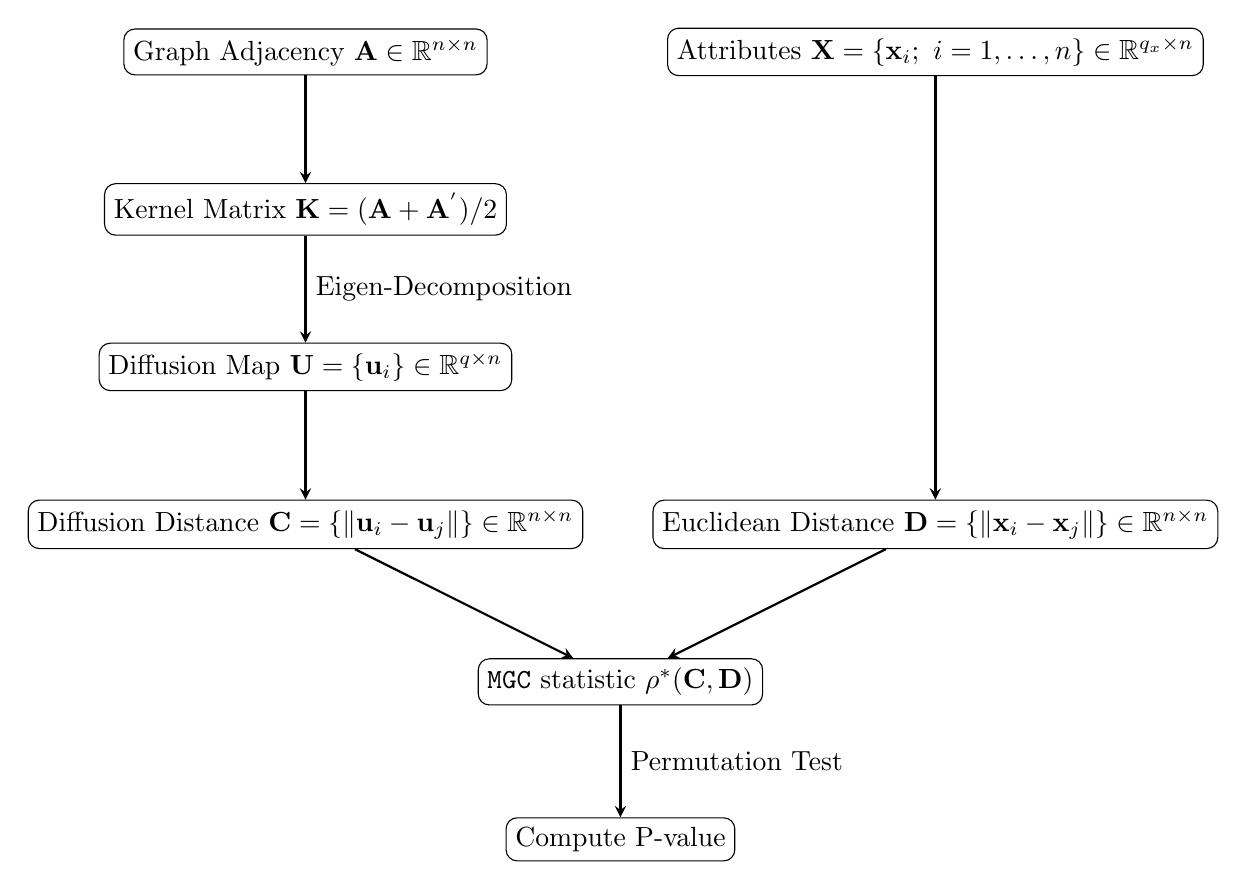
\begin{tikzpicture}[node distance=2cm]
\node (in1) [node, xshift=2cm] {Graph Adjacency $\mathbf{A} \in \mathbb{R}^{n \times n}$};
\node (in2) [node, xshift=10cm] {Attributes $\mathbf{X}=\{\mathbf{x}_{i};~i=1,\ldots,n \} \in \mathbb{R}^{q_{x} \times n}$};
\node (S1) [node, below of=in1] {Kernel Matrix $\mathbf{K}=(\mathbf{A}+\mathbf{A}^{'})/2$};

\node (S2) [node, below of=S1] {Diffusion Map $\mathbf{U}=\{\mathbf{u}_{i}\} \in \mathbb{R}^{q \times n}$};
\node (S2x) [node, below of=in2, yshift=-4cm] {Euclidean Distance $\mathbf{D}= \{\| \mathbf{x}_{i}- \mathbf{x}_{j}\|\} \in \mathbb{R}^{n \times n}$};

\node (S3) [node, below of=S2] {Diffusion Distance $\mathbf{C}= \{\| \mathbf{u}_{i}- \mathbf{u}_{j}\|\} \in \mathbb{R}^{n \times n}$};

\node (D1) [node, below of=S3, xshift=4cm] {\texttt{MGC} statistic $\rho^{*}(\mathbf{C},\mathbf{D})$};
\node (D2) [node, below of=D1] {Compute P-value};

\draw [arrow, align=right] (in1) --   (S1);
\draw [arrow] (in2) -- (S2x);
\draw [arrow] (S1) -- node[anchor=west] {Eigen-Decomposition} (S2);
\draw [arrow] (S2) -- (S3);
\draw [arrow] (S3) -- (D1);
\draw [arrow] (S2x) -- (D1);
\draw [arrow] (D1) -- node[anchor=west] {Permutation Test}(D2);
\end{tikzpicture}
\caption{Flowchart for Network Dependence Testing via Diffusion Maps and \texttt{MGC}}
\label{fig:flow}
\end{figure}

%%%%%%%%%%%%%%%%%%%%%%%%%%%%%%%%%%%%%%%%%%%%%%%%%
\subsection{Theoretical Properties}
\label{sec:theory}
Throughout this section, we assume that the parameters $t$ and $q$, and the dimension of the nodal attributes $q_x$ are fixed and finite. Moreover, we require the following distributional conditions on the graph $\mathbf{G}$ and the nodal attributes $\mathbf{X}$: 

\begin{description}[align=left]
\item [(C1)] Graph $\mathbf{G}$ is from an infinitely exchangeable graph, i.e., the adjacency matrix $\mathbf{A}$ is generated by an $n \times n$ random matrix $\mathcal{A}$ such that 
\begin{align*}
\mathcal{A}_{ij} \stackrel{d}{=} \mathcal{A}_{\sigma(i) \sigma(j)}
\end{align*}
for any $i,j=1,\ldots,n$ and any permutation $\sigma$ of size $n$, where $n$ can be finite or infinite. The notation $\stackrel{d}{=}$ stands for equality in distribution. 

\item [(C2)] The underlying distribution of the nodal attributes are of finite second moment, i.e., we assume $\{\mathbf{x}_{i};~i=1,\ldots,n\}$ are independently and identically distributed as $x$, whose second moment is finite.
\end{description}

Condition (C1) is straightforward to verify and most popular statistical networks models satisfy this condition under regularity conditions. For example, both the stochastic block model and latent position model can be thought of as a subgraph of an infinitely exchangeable random graph, when the block memberships or latent positions are assumed independently and identically distributed in each model. From condition (C1), we prove that the diffusion map $\mathbf{U}$ can furnish asymptotic conditional i.i.d. embedding for the set of nodes $V$. 

\begin{theorem}
	\label{main_lemma}
	Assume $\mathbf{G}$ satisfies (C1). Then the derived diffusion map $\{ \mathbf{u}_{i}\}$ are conditionally i.i.d. as $n \rightarrow \infty$,  i.e., there exists a latent variable $u$ such that $\mathbf{u}_{i}|u$ are i.i.d. for $i=1,\ldots,n$ as $n \rightarrow \infty$.  
\end{theorem} 

The conditional i.i.d. property of the diffusion map can lead to the consistency of distance-based correlations for the network dependence test, as long as the underlying distributions of the diffusion map and nodal attributes are of finite second moment. Therefore, condition (C2) is merely a regularity condition on the distribution of nodal attributes; while the next lemma states that the diffusion map always satisfies the finite-moment assumption.

\begin{lemma}
	\label{main_lemma_1}
    Under the same assumptions of Theorem~\ref{main_lemma}, the latent variable $u$ of the diffusion map is of finite second moment. 
\end{lemma} 

The consistency of the proposed test method is established in the next theorem.

\begin{theorem}
Assume the graph $\mathbf{G}$ and the attributes $\mathbf{X}$ satisfy condition (C1) and (C2). Then the \texttt{MGC} statistic between the derived diffusion map $\mathbf{U}$ and the nodal attributes $\mathbf{X}$ satisfies:
\begin{equation}
\rho^{*}(\mathbf{C}, \mathbf{D}) \longrightarrow 0 \mbox{ as } n \rightarrow \infty
\end{equation}
if and only if $u$ is independent of $x$. Namely, it is a consistent statistic for testing independence between the network topology and nodal attributes.
	\label{theoremMain}
\end{theorem} 

The following corollary summarizes some immediate extensions of the main testing procedure.

\begin{corollary}
\label{main_corollary}
Theorem~\ref{theoremMain} still holds, when any of the following changes are applied to the testing procedure described in Section~\ref{ssec:method}:
\begin{description}[align=left]
\item [] (1) Instead of $t=3$ and $q$ as the third elbow, $t$ and $q$ are chosen as any other finite positive integers;

\item [] (2) The nodal attributes in the input are replaced by a second graph of the same node set, which satisfies condition (C1) and has its' distance matrix $\mathbf{D}$ computed by the same diffusion map process;

\item [] (3) The \texttt{MGC} statistic in step 2 is replaced by either \texttt{dCorr} or \texttt{mCorr}.
\end{description}
\end{corollary}

Namely, the theoretical consistency always holds regardless of the choice on $t$ and $q$; the same approach can be applied to test dependency between graphs of arbitrary structures, e.g., testing between a weighted directed graph and an unweighted undirected graph, by deriving the diffusion distance for each graph individually; that is, once the appropriate distance is determined, distance-based measures other than \texttt{MGC} can also be consistent, such as \texttt{dCorr} and \texttt{mCorr}. 

Therefore, we offer more discussions on the parameter selection in the next section, suggest a two-graph testing scenario, and use \texttt{mCorr} and \texttt{HHG} in the simulations to further make a comparison with the main approach.

All proofs are supplied in Appendix~\ref{ssec:proof}.

\subsection{Discussions}
\label{ss:dis}
 
In this section, we discuss the parameter selection and the advantages of diffusion maps over other embeddings. Note that the advantages of \texttt{MGC} is extensively demonstrated in \cite{shen2016discovering}.

There are two parameters to choose for the diffusion map, i.e., the time step $t$, and the dimension of graph embedding $q$. Theoretical properties always hold for finite $t$ and $q$, but their choices may affect the testing power. Empirically, it turns out that the diffusion map is relatively insensitive to choice of $t$, and able to well capture the geometric structure in a wide range of $t>1$, from which we choose to fix $t=3$ throughout; upon fixing $t$, the diffusion distance is also relatively indifferent to the choice of $q$, for which we opt to select $q$ as the third elbow of the eigenvalue scree plot by the profile likelihood method from~\cite{ZhuGhodsi2006}. This is a widely-used automatic algorithm for selecting the number of important features, whenever eigenvalues or singular values are involved. 

To support our parameter choices, we provide empirical evidence in Figure~\ref{fig:diffusions}: an adjacency matrix of $n=100$ is generated by the three-block stochastic block model in Equation~\ref{eq:Three} (details in Section~\ref{sec:simulation}), followed by the diffusion distances at different $t$ and $q$. The diffusion distance matrix is always able to preserve the block structures for $t \in [2,10]$ and $q \in [2,n]$. Recognizing such block structures is important in detecting dependence between the graph structure and block membership.

In comparison, standard graph embedding methods are often sensitive to the choice of $q$. Figure~\ref{fig:embedding} shows the Euclidean distance of the adjacency spectral embedding (ASE) \cite{SussmanEtAl2012} applied to the same adjacency matrix. For ASE, the correct dimensional choice equals the number of blocks, i.e., the distance matrix at $q=3$ shows a clear block structure. However, a slight mis-specification of $q$ can cause the embedding to have a more obscure block structure, and the elbow method often fails to find the correct $q$ for ASE.

\begin{figure}[!ht]
	\centering
	\begin{subfigure}[b]{0.23\textwidth}
		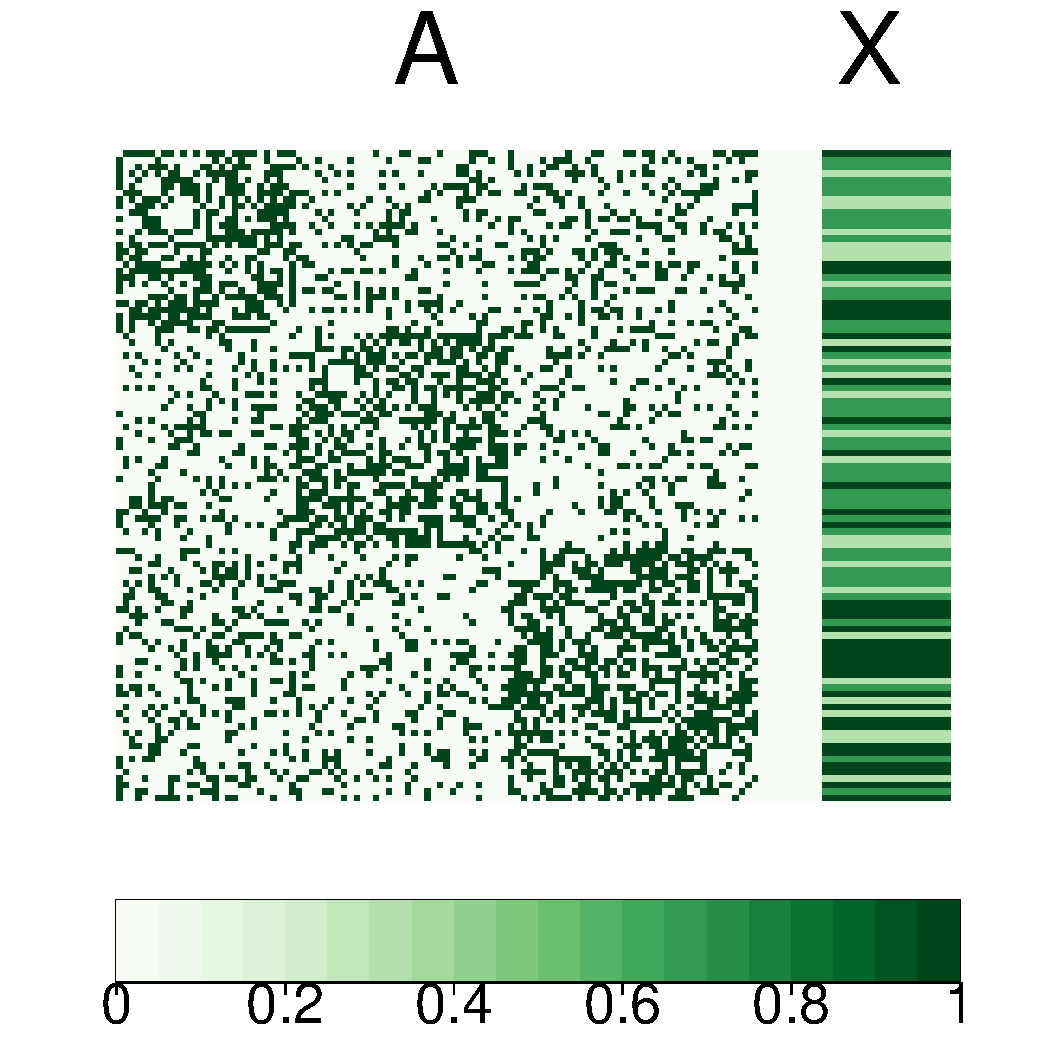
\includegraphics[width=\textwidth]{../Figure/Amat.pdf}
		\caption{}
		\label{fig:a}
	\end{subfigure}
	\begin{subfigure}[b]{0.23\textwidth}
		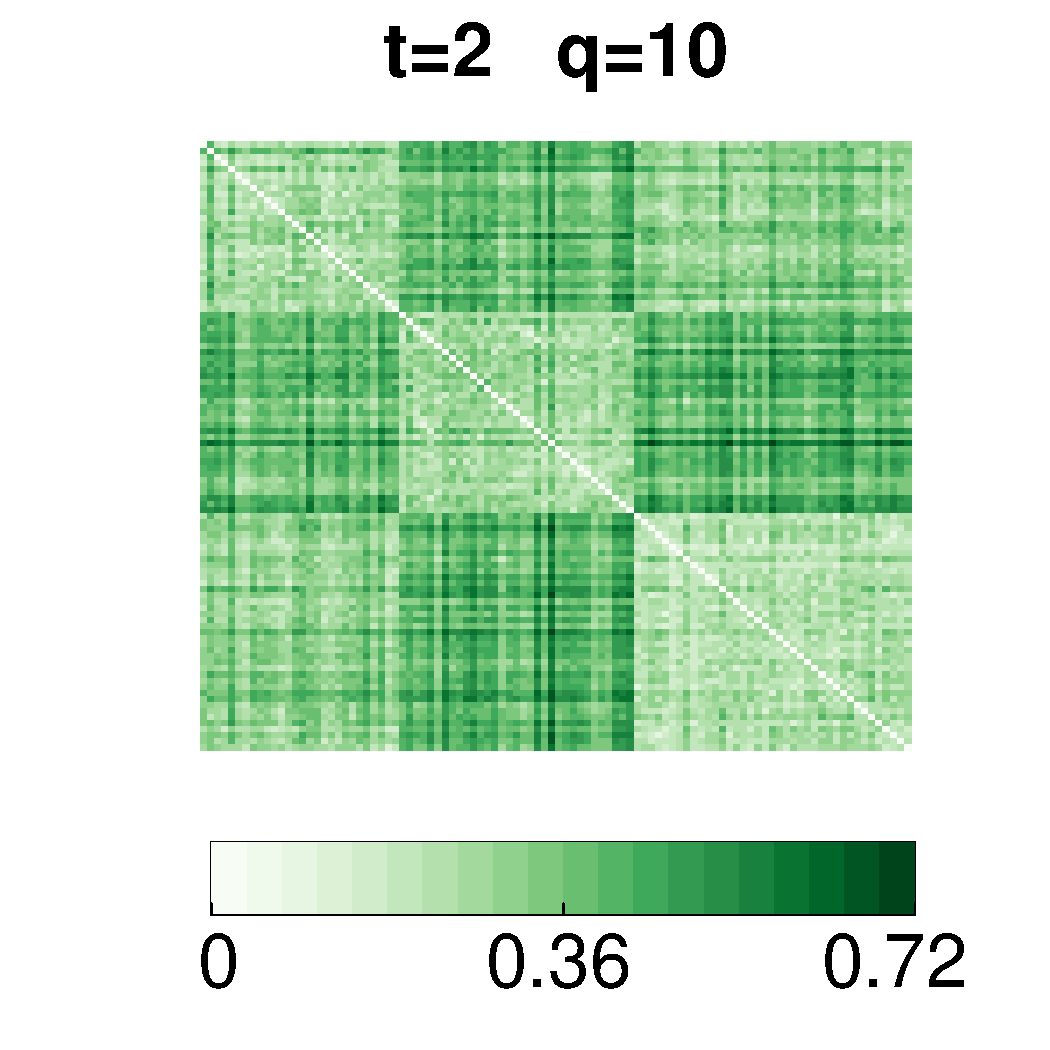
\includegraphics[width=\textwidth]{../Figure/Q10T2.pdf}
		\caption{}
		\label{fig:b}
	\end{subfigure}
	\begin{subfigure}[b]{0.23\textwidth}
		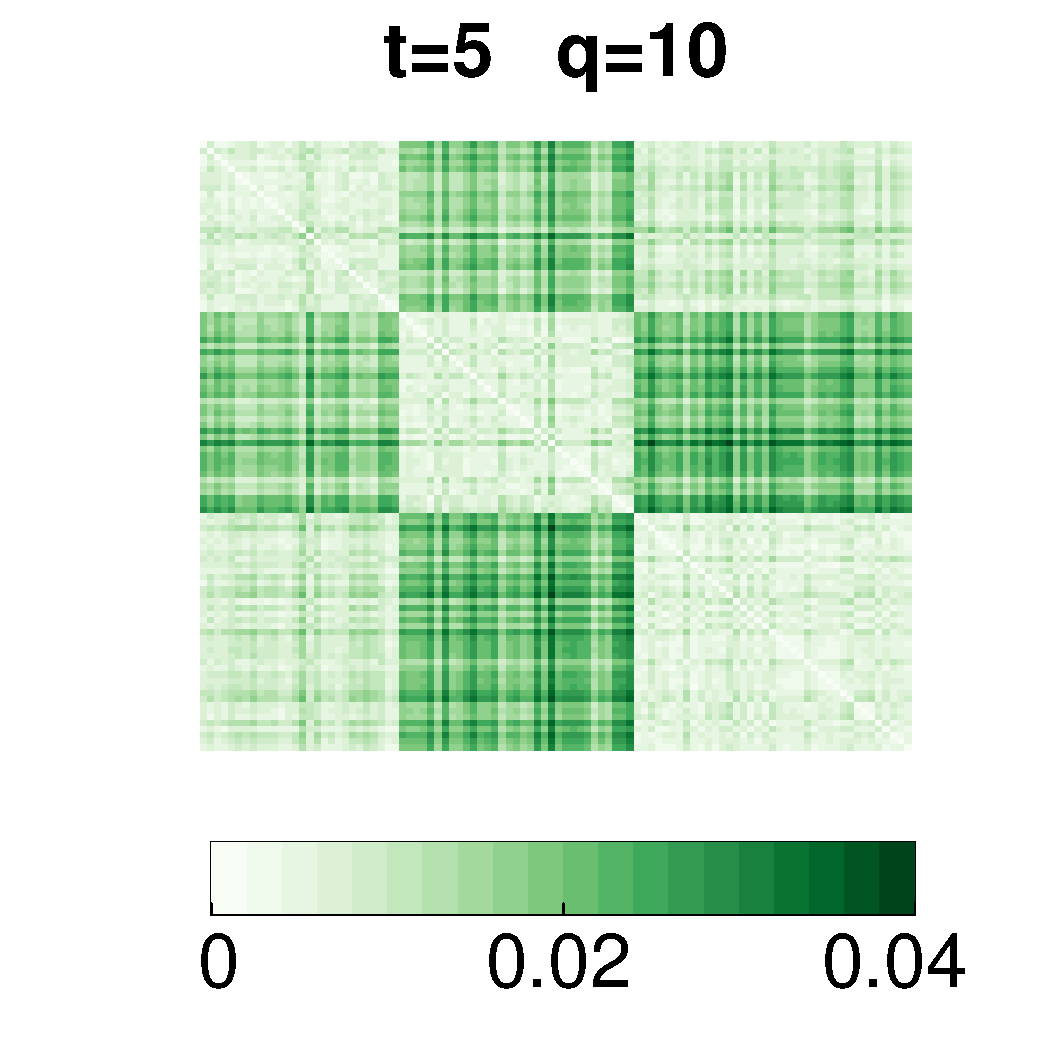
\includegraphics[width=\textwidth]{../Figure/Q10T5.pdf}
		\caption{}
		\label{fig:c}
	\end{subfigure}
	\begin{subfigure}[b]{0.23\textwidth}
		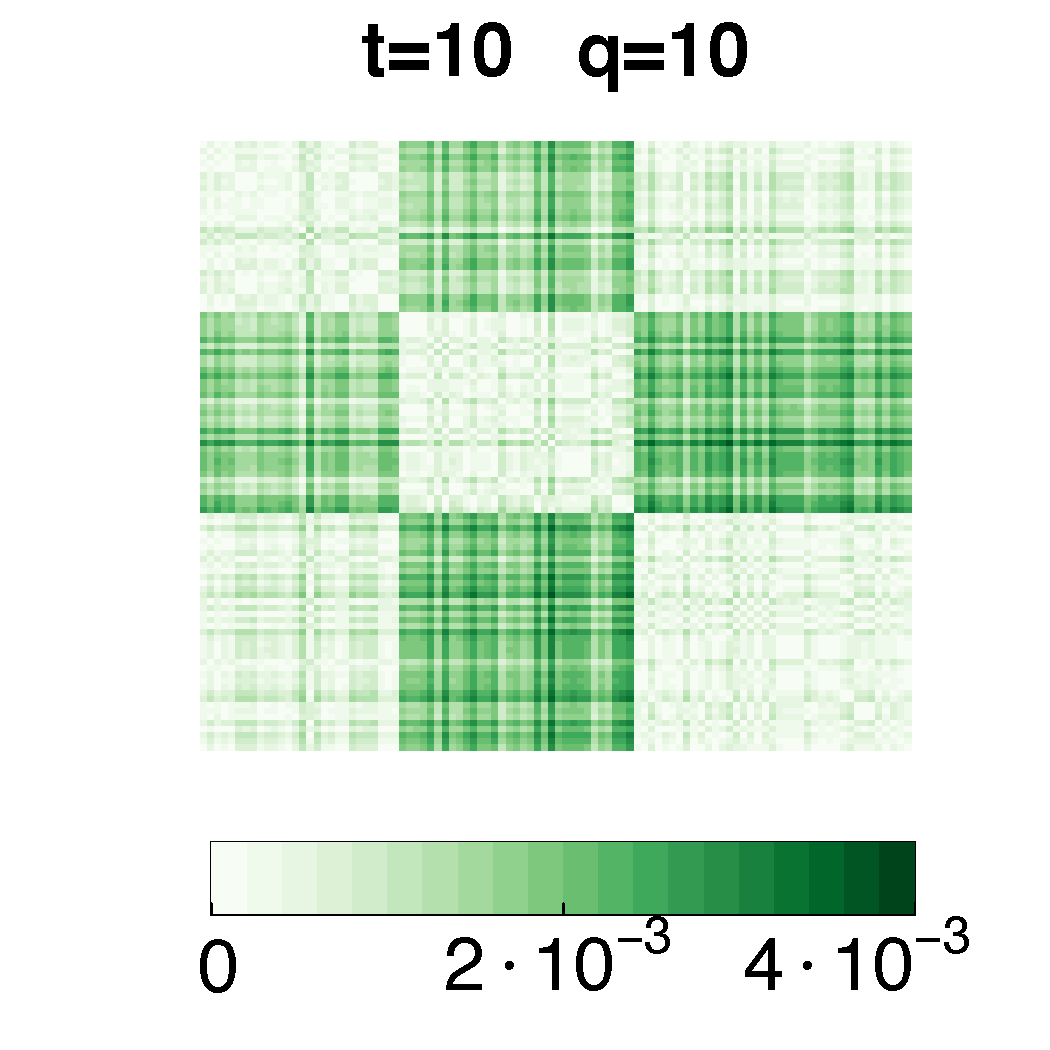
\includegraphics[width=\textwidth]{../Figure/Q10T10.pdf}
		\caption{}
		\label{fig:d}
	\end{subfigure}
    \\ \bigskip
	\begin{subfigure}[b]{0.23\textwidth}
		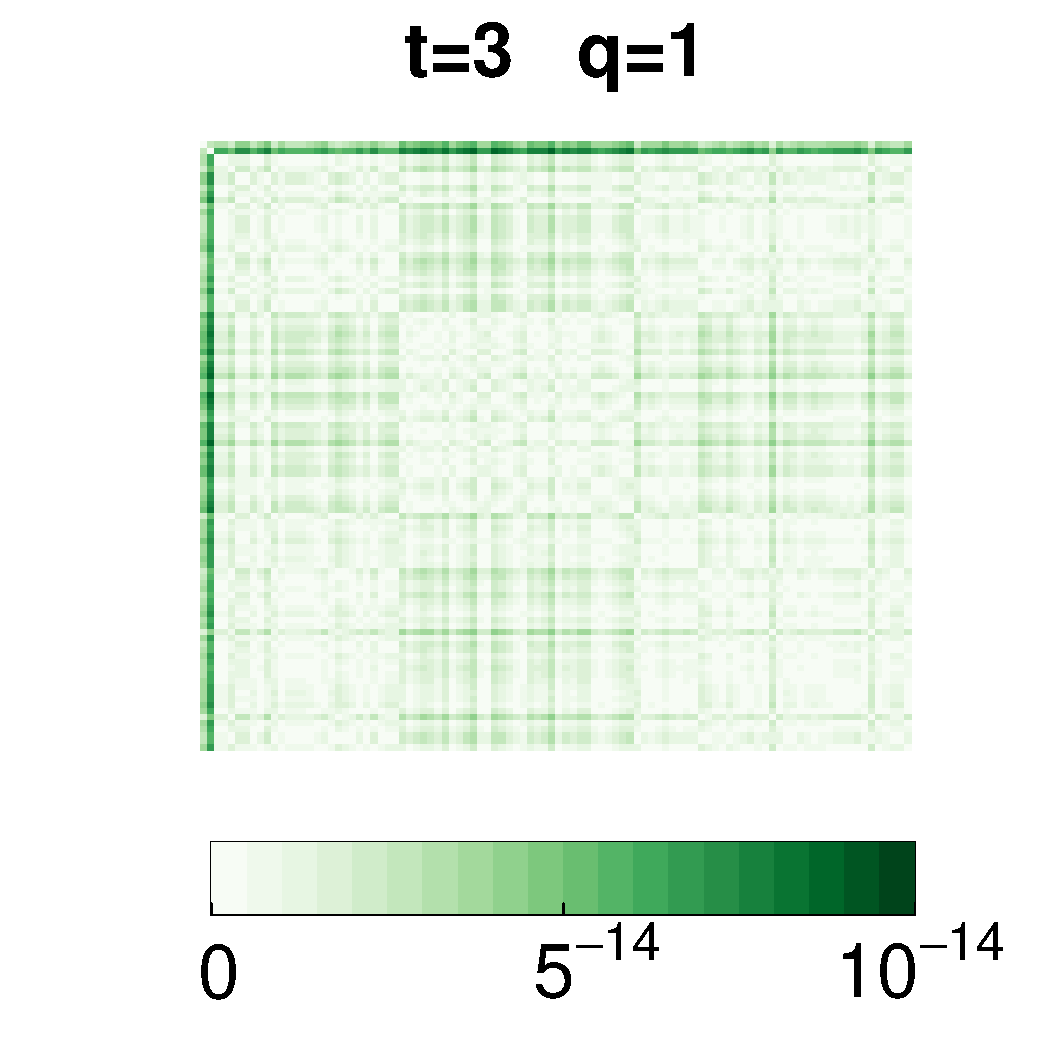
\includegraphics[width=\textwidth]{../Figure/Q1T3.pdf}
		\caption{}
		\label{fig:q1}
	\end{subfigure}
	\begin{subfigure}[b]{0.23\textwidth}
		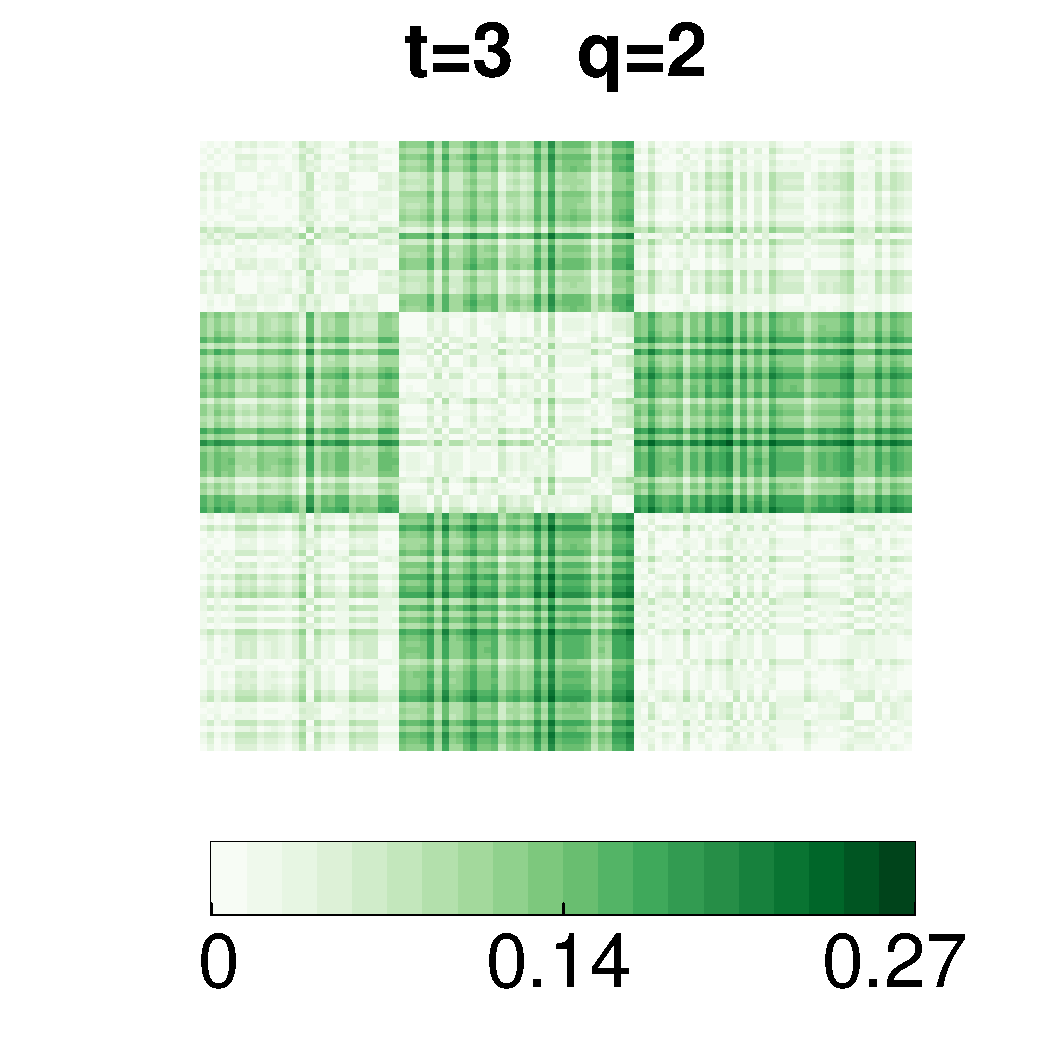
\includegraphics[width=\textwidth]{../Figure/Q2T3.pdf}
		\caption{}
		\label{fig:q2}
	\end{subfigure}
	\begin{subfigure}[b]{0.23\textwidth}
		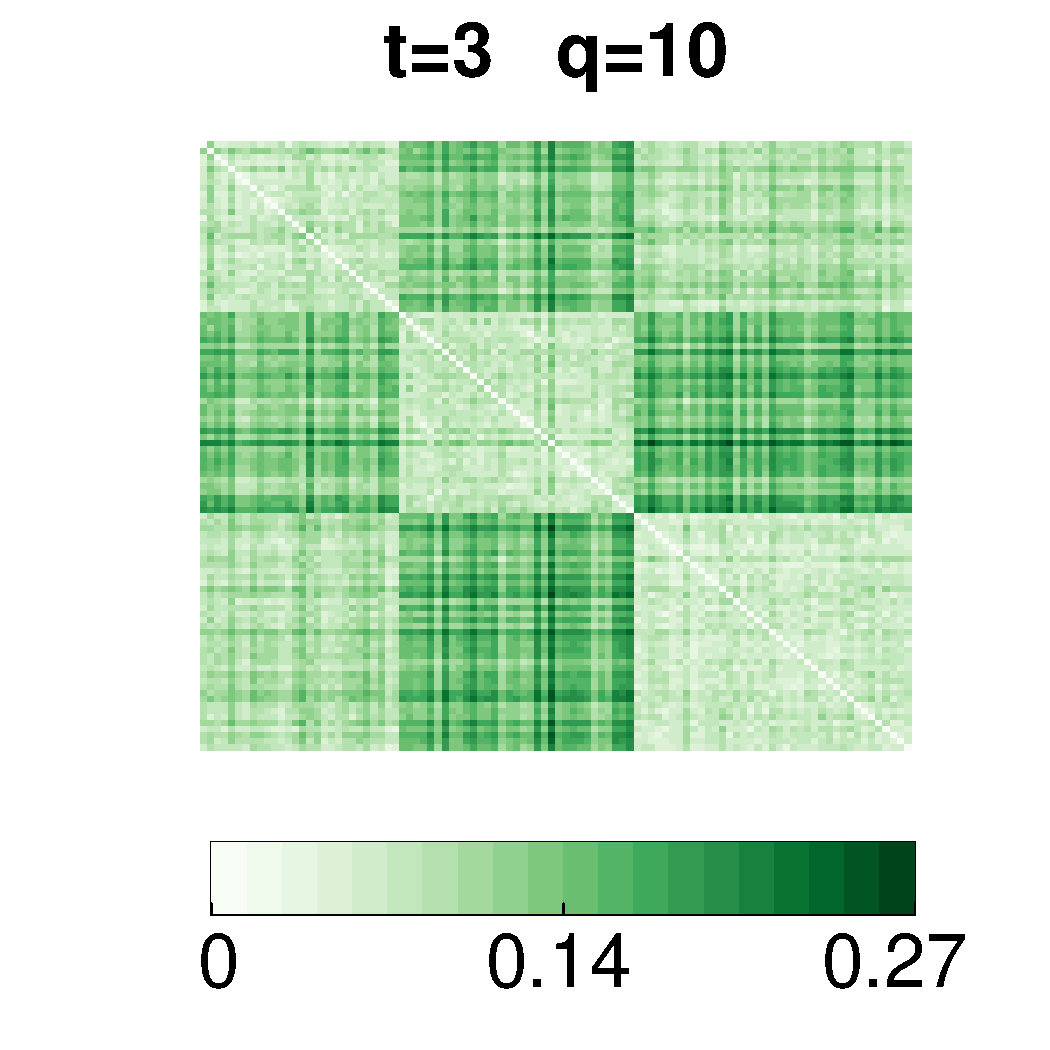
\includegraphics[width=\textwidth]{../Figure/Q10T3.pdf}
		\caption{}
		\label{fig:q5}
	\end{subfigure}
	\begin{subfigure}[b]{0.23\textwidth}
		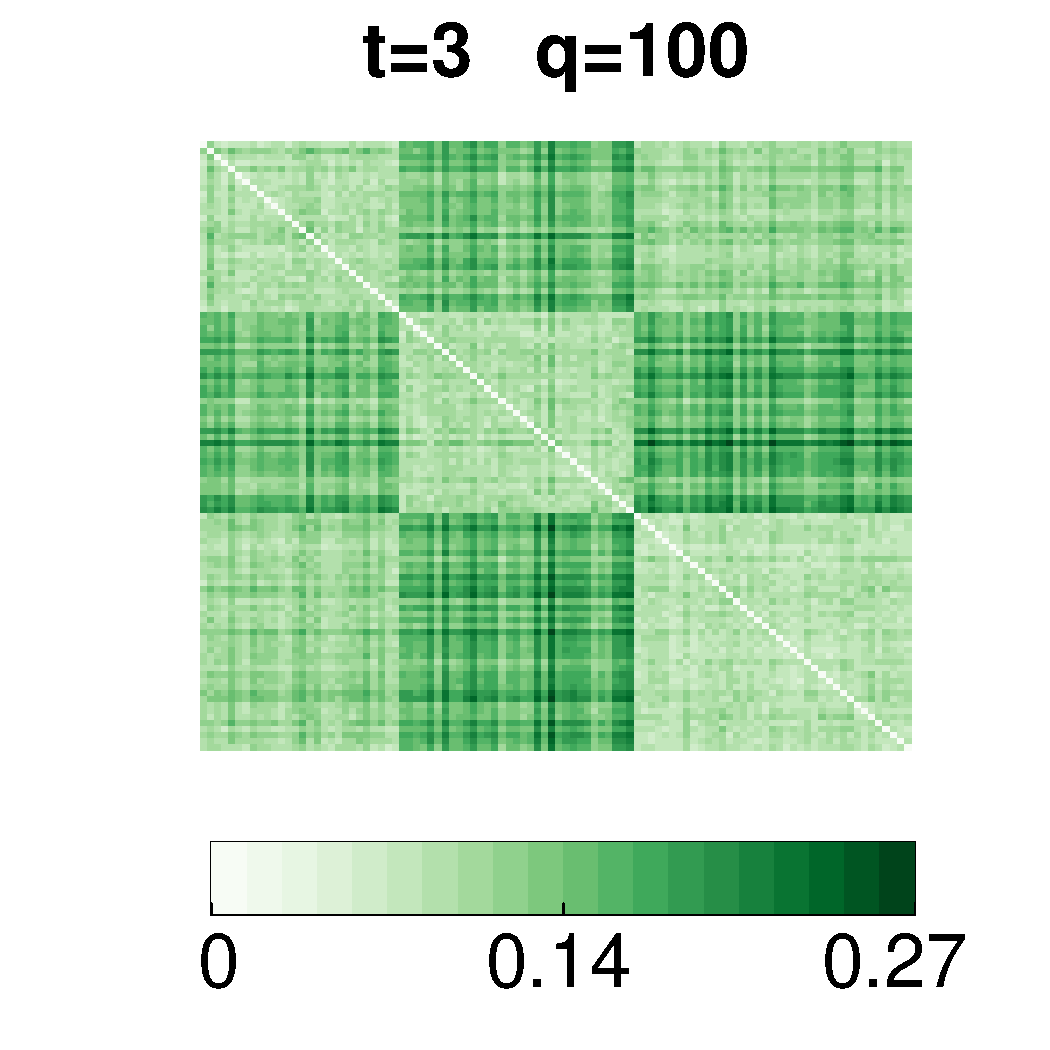
\includegraphics[width=\textwidth]{../Figure/Q100T3.pdf}
		\caption{}
		\label{fig:q10}
	\end{subfigure}
	\caption{Diffusion maps are robust against parameter mis-specifications. Panel (a) illustrates the three-block adjacency matrix $\mathbf{A}$ generated by Equation~\ref{eq:Three}. Panel (b)-(d) show the diffusion distance matrix at $q=10$ and increasing $t$, while panel (e)-(h) present the diffusion distance at $t=3$ and increasing $q$. The distance matrix exhibits a clear block structure, for $t \in [2,10]$ and $q \in [2,n]$. Note that at $t=3$, the first three elbows of eigenvalues are $(1,3,84)$ respectively.}
	\label{fig:diffusions}
\end{figure}

\begin{figure}[!ht]
	\centering
	\begin{subfigure}[b]{0.23\textwidth}
	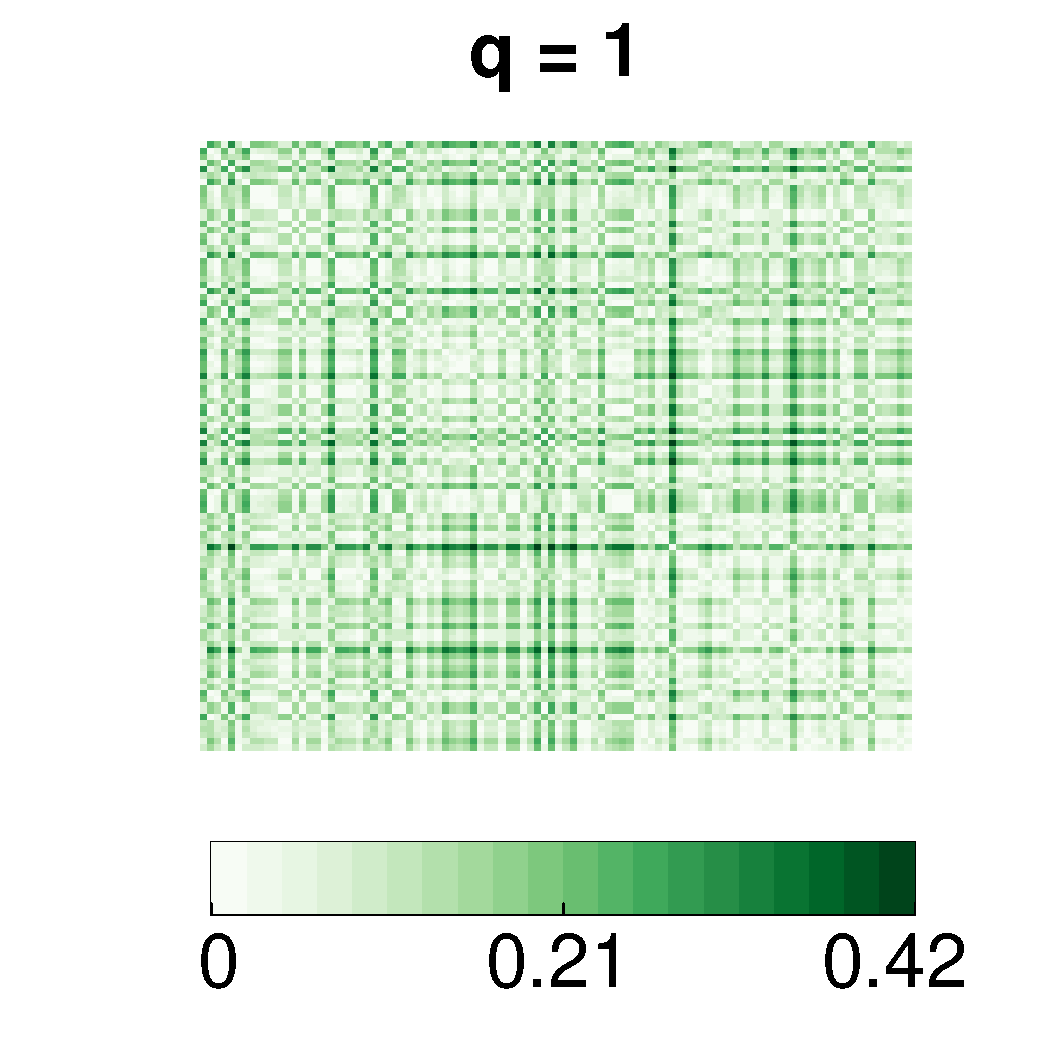
\includegraphics[width=\textwidth]{../Figure/E1.pdf}
	\caption{}
	\label{fig:e1}
	\end{subfigure}
	\begin{subfigure}[b]{0.23\textwidth}
	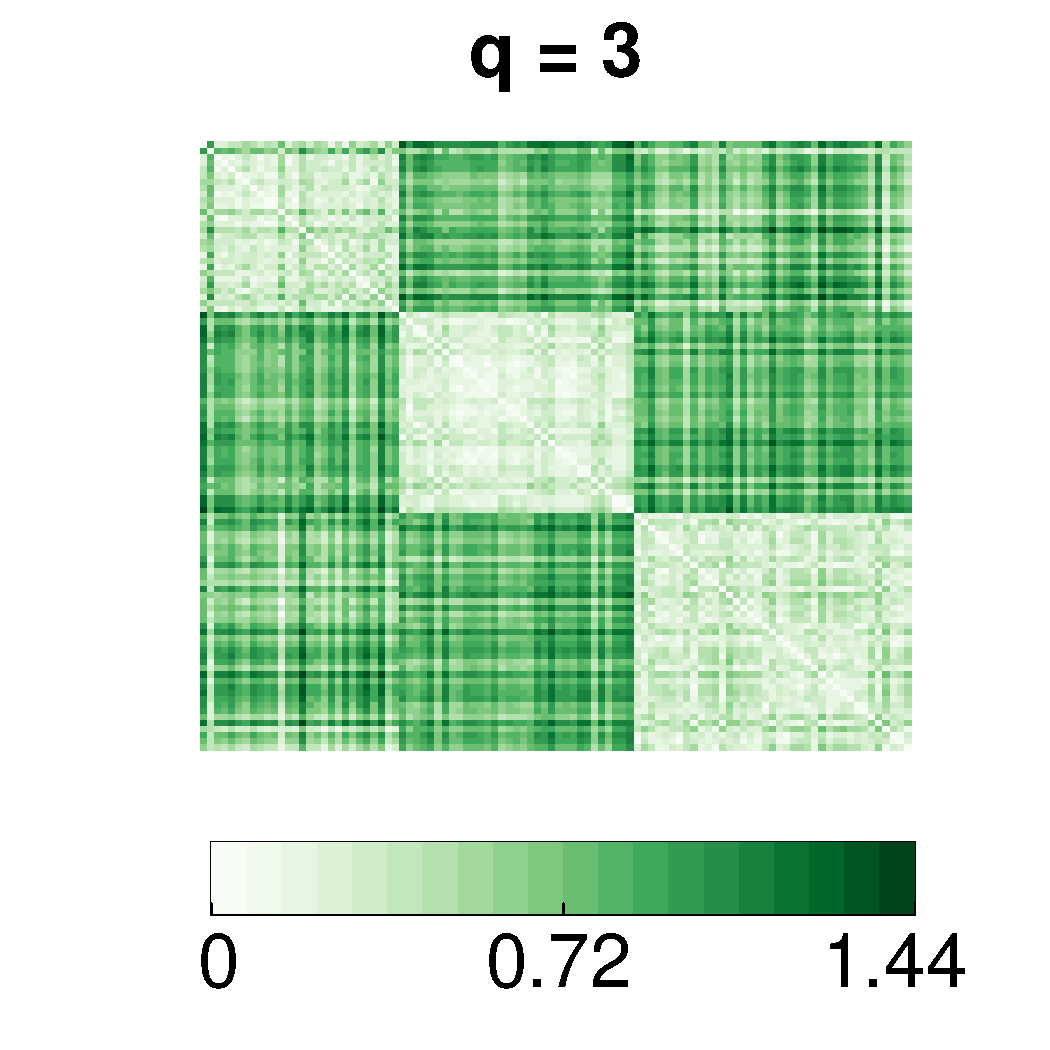
\includegraphics[width=\textwidth]{../Figure/E3.pdf}
	\caption{}
	\label{fig:e3}
	\end{subfigure}
	\begin{subfigure}[b]{0.23\textwidth}
	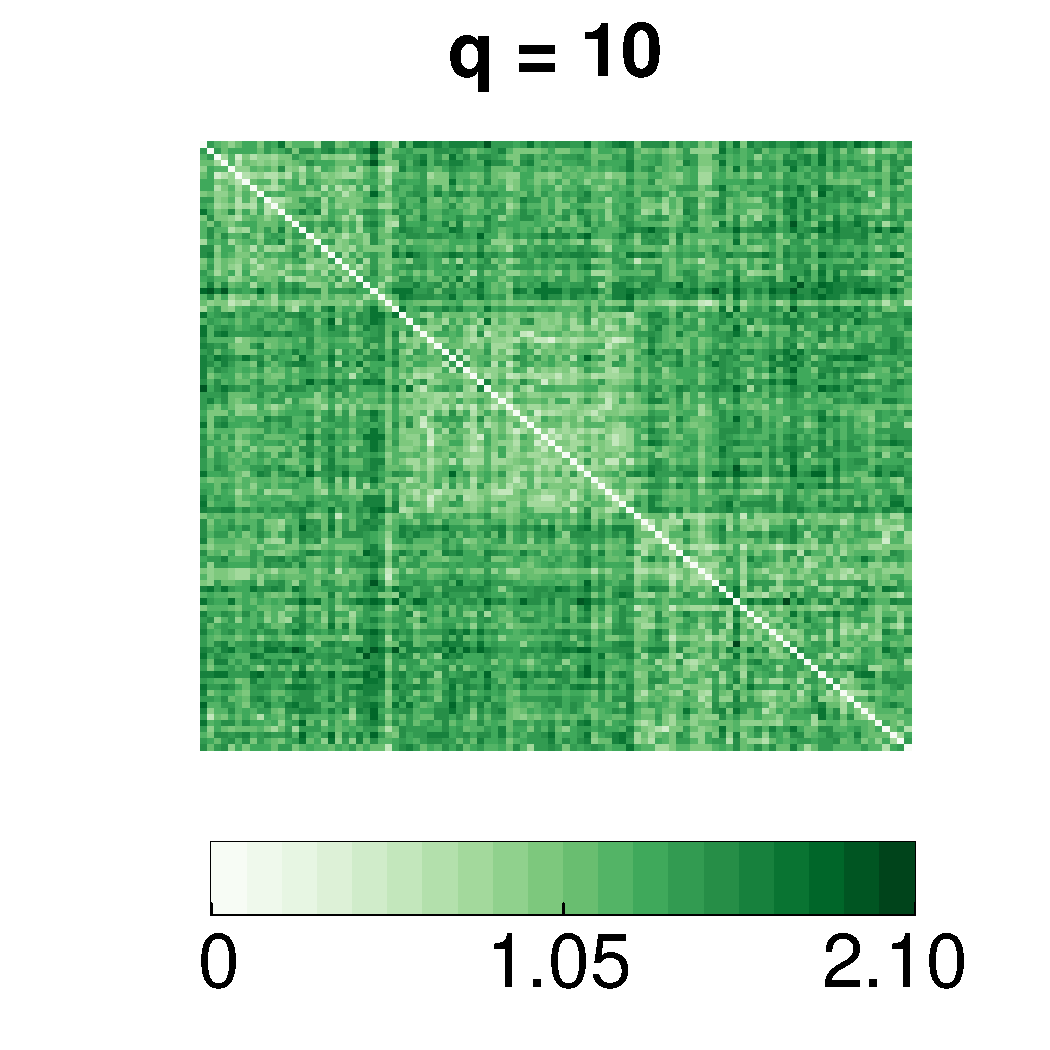
\includegraphics[width=\textwidth]{../Figure/E10.pdf}
	\caption{}
	\label{fig:e10}
	\end{subfigure}
	\begin{subfigure}[b]{0.23\textwidth}
	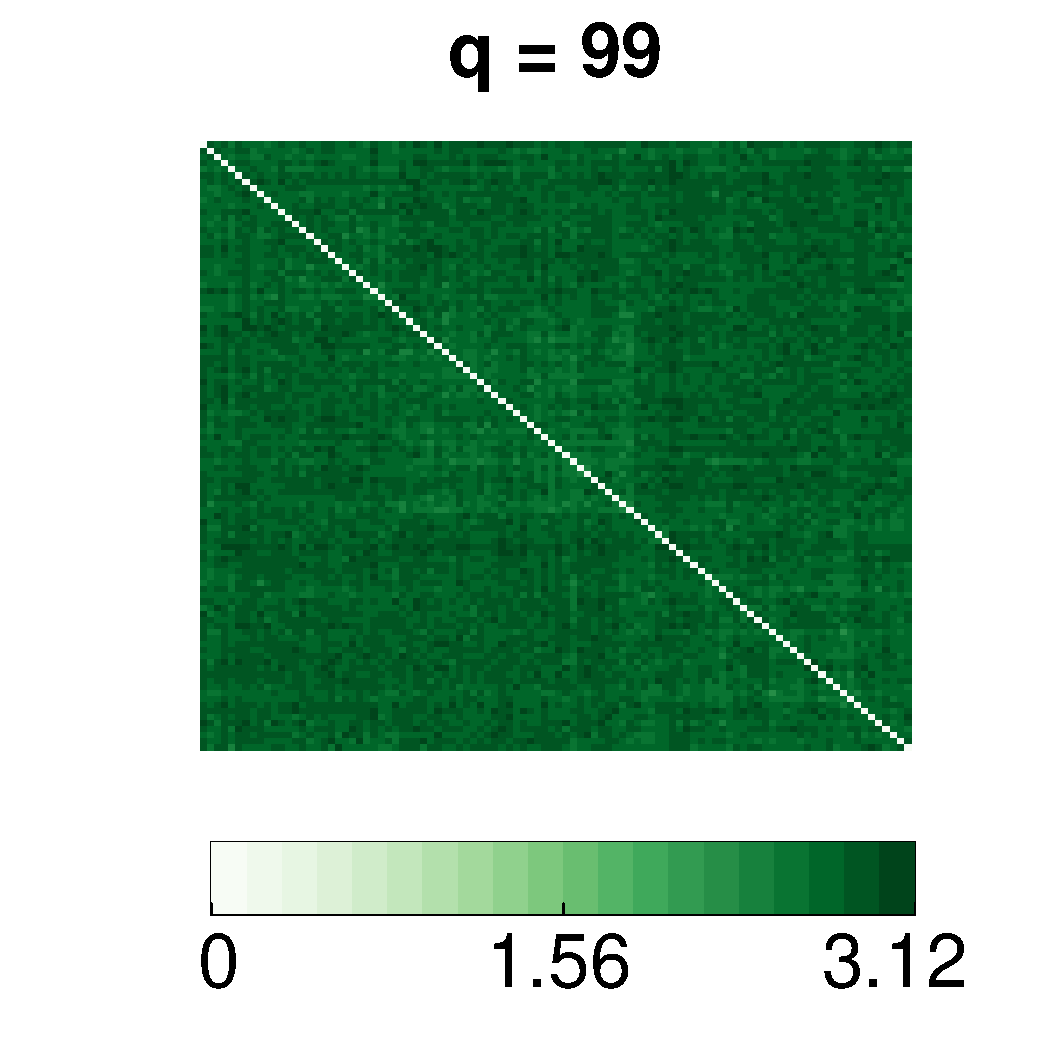
\includegraphics[width=\textwidth]{../Figure/E99.pdf}
	\caption{}
	\label{fig:e99}
	\end{subfigure}
	\caption{Adjacency spectral embedding is not robust against dimension misspecification particularly compared to the diffusion maps. Panel (a)-(d) show the Euclidean distance matrix of ASE at increasing $q$, using the same adjacency matrix in Figure~\ref{fig:diffusions}(a). Only ASE at $q=3$, namely the correct dimension, is able to display a clear block structure. Note that the first three elbows are $(1,45,70)$, so that it is difficult for ASE to recognize the block structure when the dimension is chosen via the scree plot.}
\label{fig:embedding}
\end{figure}

Therefore, our motivation to use diffusion maps is three-fold: it yields an embedding of the graph structure into the Euclidean space; it is relatively robust against parameter mis-specification; and it allows a seamless integration with distance-based correlations for consistent dependency testing. On the other hand, it is tempting to use other embedding methods, like adjacency spectral embedding, Laplacian spectral embedding \cite{rohe2011spectral}, the latent factor embedding \cite{fosdick2015testing}, etc. Those embeddings can also be directly combined with \texttt{dCorr} or \texttt{MGC} to test dependence, but they may lose the theoretical properties without more strict model assumption and are often more sensitive to the parameter choice, thereby leading to sub-optimal performance. For comparison purposes, we include other embedding choices for benchmark in the simulations.


%%%%%%%%%%%%%%%%%%%%%%%%%%%%%%%%%%%%%%%%%%%%%%%%%%
\section{Numerical Studies}
\label{sec:simulation}

In this section, we demonstrate the advantages of our approach via simulations and real data experiment. Throughout the numerical studies, we mainly compare our approach to the likelihood ratio test proposed by Fosdick and Hoff (\texttt{FH})~\cite{fosdick2015testing}, as well as a number of variants mentioned in Section~\ref{sec:method}: in place of \texttt{MGC}, we consider applying \texttt{mCorr} and \texttt{HHG} to the distances; and instead of diffusion distance as the network metric, we consider using the Euclidean distances of the adjacency matrix (\texttt{AM}) or the latent factors (\texttt{LF}), prior to computing the distance-based correlation. Our main approach is denoted as $\texttt{MGC} \circ \texttt{DM}$ (\texttt{MGC} statistic applied to diffusion maps), whereas the other variants are denoted as $\texttt{MGC} \circ \texttt{AM}$, $\texttt{mCorr} \circ \texttt{DM}$, $\texttt{HHG} \circ \texttt{LF}$, etc. 

For each simulation, we generate sample graph and the corresponding attributes, carry out the permutation test for each method, and reject the null if the resulting p-value is less than $\alpha = 0.05$. The testing power of each method equals the percentage of correct rejection out of $500$ Monte-Carlo replicates, and a higher power implies a better method. For the real data experiment, we directly report the p-value of the permutation test, since the testing power is not available, and a lower p-value indicates a better method assuming the existence of relationships. 

Whenever dimension selection is required, i.e., selection of $q$ for \texttt{DM} and \texttt{LF}, we always pick the third elbow of the scree plot bounded above by $\min(n, 100)$. 

\subsection{Stochastic Block Model}

The first simulation generates graphs by the stochastic block model (SBM), which is one of the most popular network models which many network methodologies have been built on. The SBM assumes that each of $n$ nodes in $\mathbf{G}$ must belong to one of $K \in \mathbb{N}$ blocks, and determines the edge probability based on the block affiliations of the connecting nodes: For $i=1,\ldots,n$, assume that a latent variable of $\mathbf{z}_{i} \overset{i.i.d.}{\sim} Multinomial\big( \pi_{1}, \pi_{2}, ... , \pi_{K} \big)$ denotes the block membership of each node, and $p_{kl} \in [0,1]$ implies the edge probability between any two nodes of class $k$ and $l$ respectively; then the upper triangular entries of $\mathbf{A}$ are independent and identically distributed conditioned on $\{\mathbf{z}_{i}\}$:
\begin{equation} 
\mathbf{A}_{ij} \big| \mathbf{z}_{i}, \mathbf{z}_{j} \overset{i.i.d.}{\sim} Bernoulli\big( \sum\limits_{k,l=1}^{K} p_{kl} \mathbf{I} \big( \mathbf{z}_{i} = k, \mathbf{z}_{j} = l  \big)    \big); \quad \forall  i < j,
\end{equation}
where $\mathbf{I}(\cdot)$ is the indicator function. %We consider the undirected, unweighted, and no self-loop version of SBM.

It is of common interest to detect whether the block structure has anything to do with the graph connectivity; and noisy information on the block structure often better reflects reality and adds difficulty to the testing. Thus we consider testing dependency between the graph having the adjacency matrix $\mathbf{A}$ and a noisy block membership $\mathbf{X}$, which are correlated through true block memberships $\mathbf{Z}$. We set $n=100$ and $K=3$, select $\mathbf{z}_i$ uniformly from $\Omega=\{1,2,3\}$ for each $i$, generate the edge probability by
\begin{equation}
\label{eq:Three}
E(\mathbf{A}_{ij} | \mathbf{z}_{i}, \mathbf{z}_{j}) = 0.5 \mathbf{I}(|\mathbf{z}_{i} - \mathbf{z}_{j}| = 0) + 0.2 \mathbf{I}(|\mathbf{z}_{i} - \mathbf{z}_{j}| = 1) + 0.3 \mathbf{I}(|\mathbf{z}_{i} - \mathbf{z}_{j}| = 2), \quad i,j = 1, \ldots, n,
\end{equation} 
and contaminate the true block membership by: for each $i$, $\mathbf{x}_{i}=\mathbf{z}_{i}$ with probability $0.5$, and equally likely to take other values in $\Omega$, i.e., the true block memberships are observed half of the time.

Namely, within-block edge probability is always $0.5$, while between-block edge probability is $0.2$ when the block labels differ by $1$, and $0.3$ when the block labels differ by $2$. A visualization of the sample data is shown in Figure~\ref{fig:diffusions}. 
Notably, although within-block edge probability is the largest, the between-block edge probability is not linearly related to the distance of the block-memberships, i.e., the edge probability between a node of block $1$ and a node of block $3$ is higher than the edge probability between block $1$ and block $2$. 

Therefore, this three-block SBM generates a noisy and nonlinear dependency structure between $\mathbf{A}$ and $\mathbf{X}$, for which \texttt{MGC} is expected to work better than \texttt{mCorr}, \texttt{HHG}, and the standard likelihood ratio test; moreover, the diffusion map should be more robust than the other two metrics of adjacency matrix (\texttt{AM}) and latent factors (\texttt{LF}). Indeed, Figure~\ref{fig:diffusions} shows that the main approach (i.e., \texttt{MGC} $\circ$ \texttt{DM}) prevails in the testing powers among all the methods.

\begin{SCfigure}[][ht]
	\centering
	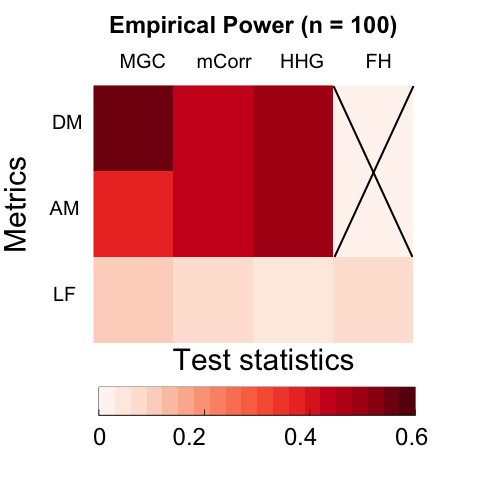
\includegraphics[width=0.4\paperwidth, height=0.4\paperwidth]{../Figure/ThreeSBM_Elbow3.png}
	\caption{The power heatmap under the three-block SBM (Equation~\ref{eq:Three}) demonstrates that for all possible combinations of test statistics with distance metrics, \texttt{MGC} with the diffusion maps (\texttt{DM}) provides the best power compared to all other methods.}
	\label{fig:threeSBM}
\end{SCfigure}

\subsection{SBM with Linear and Nonlinear Dependencies}

To better illuminate the advantage of our main approach under different scenarios, here we use the same three-block SBM and its block memberships $\{ \mathbf{z}_{i} : i=1,2, \ldots, n=100 \}$ as in the last section, except that the edge probability is now controlled by $\theta \in (0, 1)$ as follows:
\begin{equation}
E(\mathbf{A}_{ij} | \mathbf{z}_{i}, \mathbf{z}_{j}) = 0.5 \mathbf{I}(|\mathbf{z}_{i} - \mathbf{z}_{j}| = 0) + 0.2 \mathbf{I}(|\mathbf{z}_{i} - \mathbf{z}_{j}| = 1) + \theta \mathbf{I}(|\mathbf{z}_{i} - \mathbf{z}_{j}| = 2); \quad i,j = 1, \ldots, n.
\label{eq:mono}
\end{equation}
The noisy block memberships $\mathbf{X}$ is generated in the same way as before.

When $\theta = 0.2$, the three-block SBM is the same as a two-block SBM, where within-block edge probability equals $0.5$ while the between-block edge probability is always $0.2$, i.e., it represents a linear association between the adjacency matrix and the block membership; when $\theta<0.2$, the association is still close to linear; when $\theta > 0.2$ and gets further away, the relationship becomes strongly nonlinear.

Figure~\ref{fig:powerplot} plots the power against $\theta$ of \texttt{DM} based on all methods. All of \texttt{MGC}, \texttt{mCorr}, and \texttt{HHG} perform almost the same at linear or close to linear dependency (i.e, $\theta \leq 0.2$), with \texttt{MGC} being significantly more powerful as the dependency shifts to strongly nonlinear. This observation confirms that the \texttt{MGC} is able to capture nonlinear dependencies in network testing, suggesting it is a better test statistic for general usage.

\begin{figure}[!ht]
	\centering
	\begin{subfigure}[b]{0.7\textwidth}
		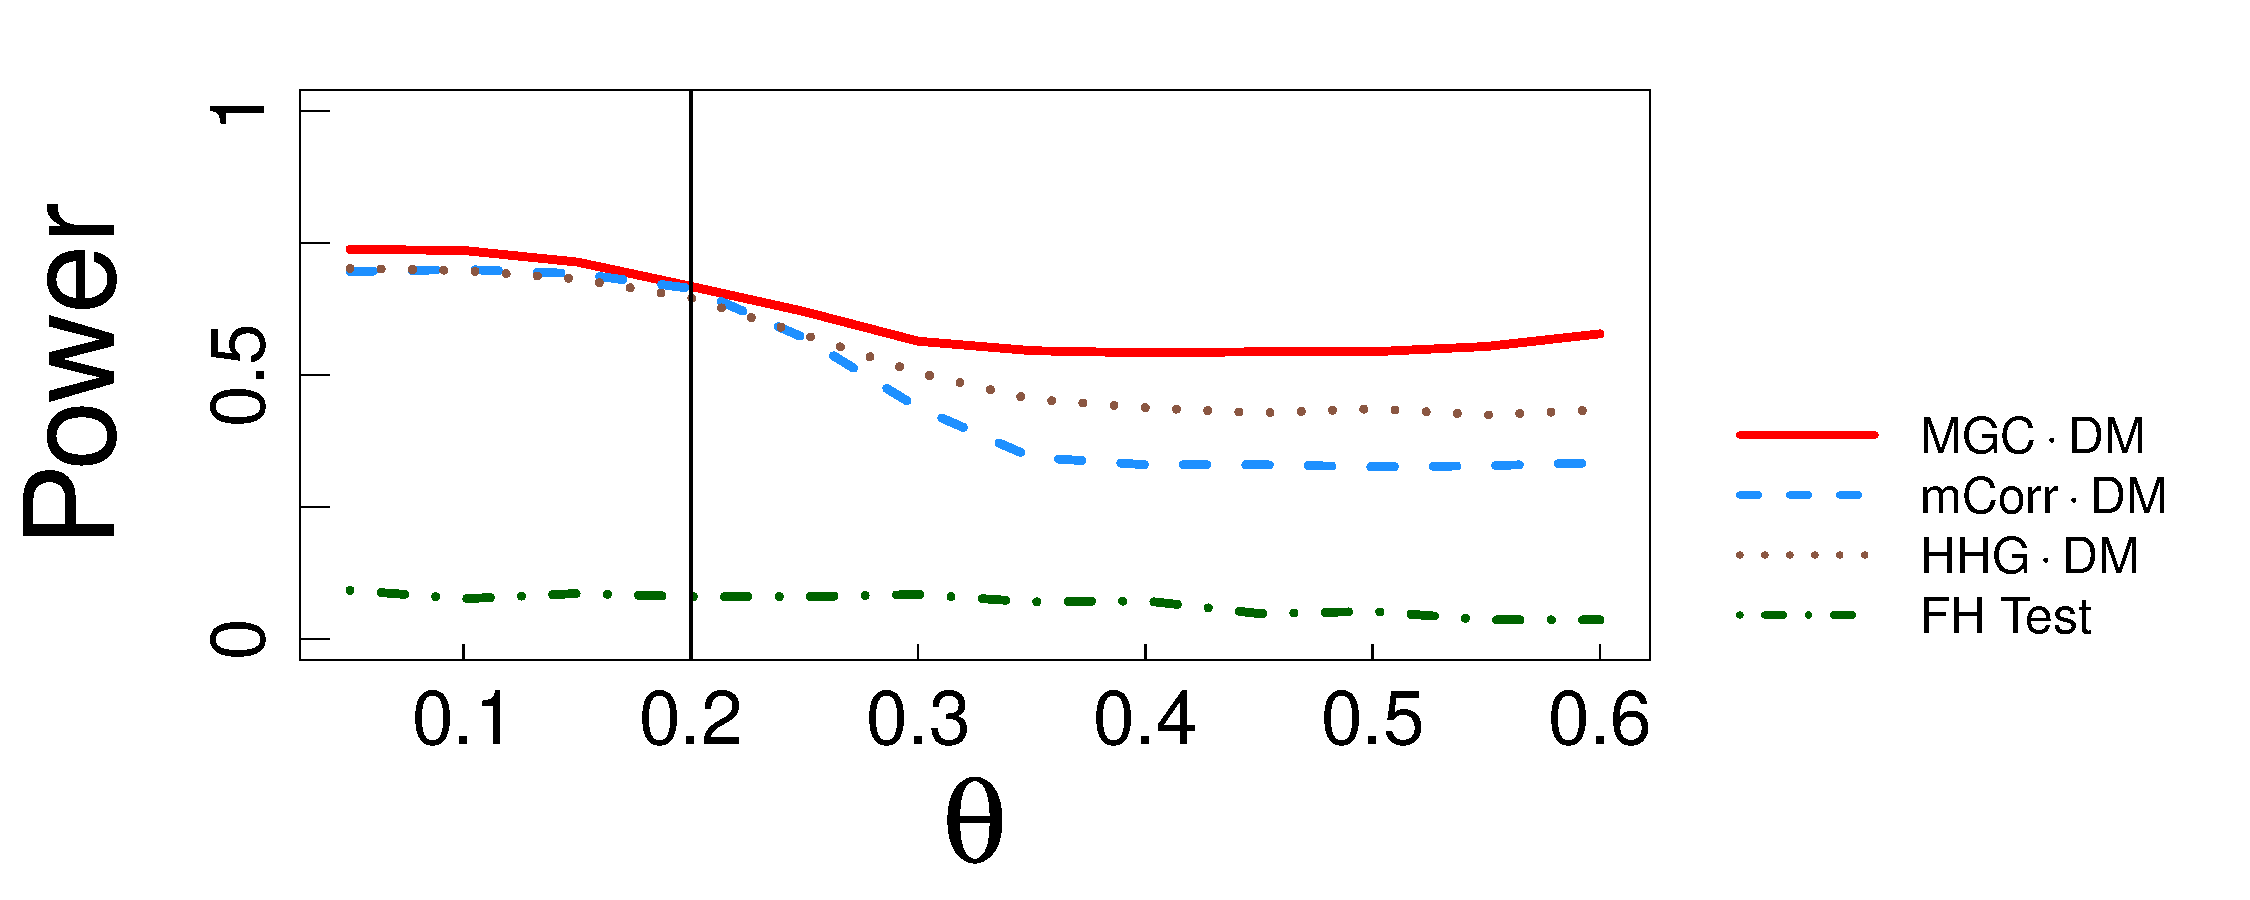
\includegraphics[width=\textwidth]{../Figure/monoelbow3_t3.pdf}
		\caption{} 
		\label{fig:powerplot}
	\end{subfigure}
	\begin{subfigure}[b]{0.7\textwidth}
		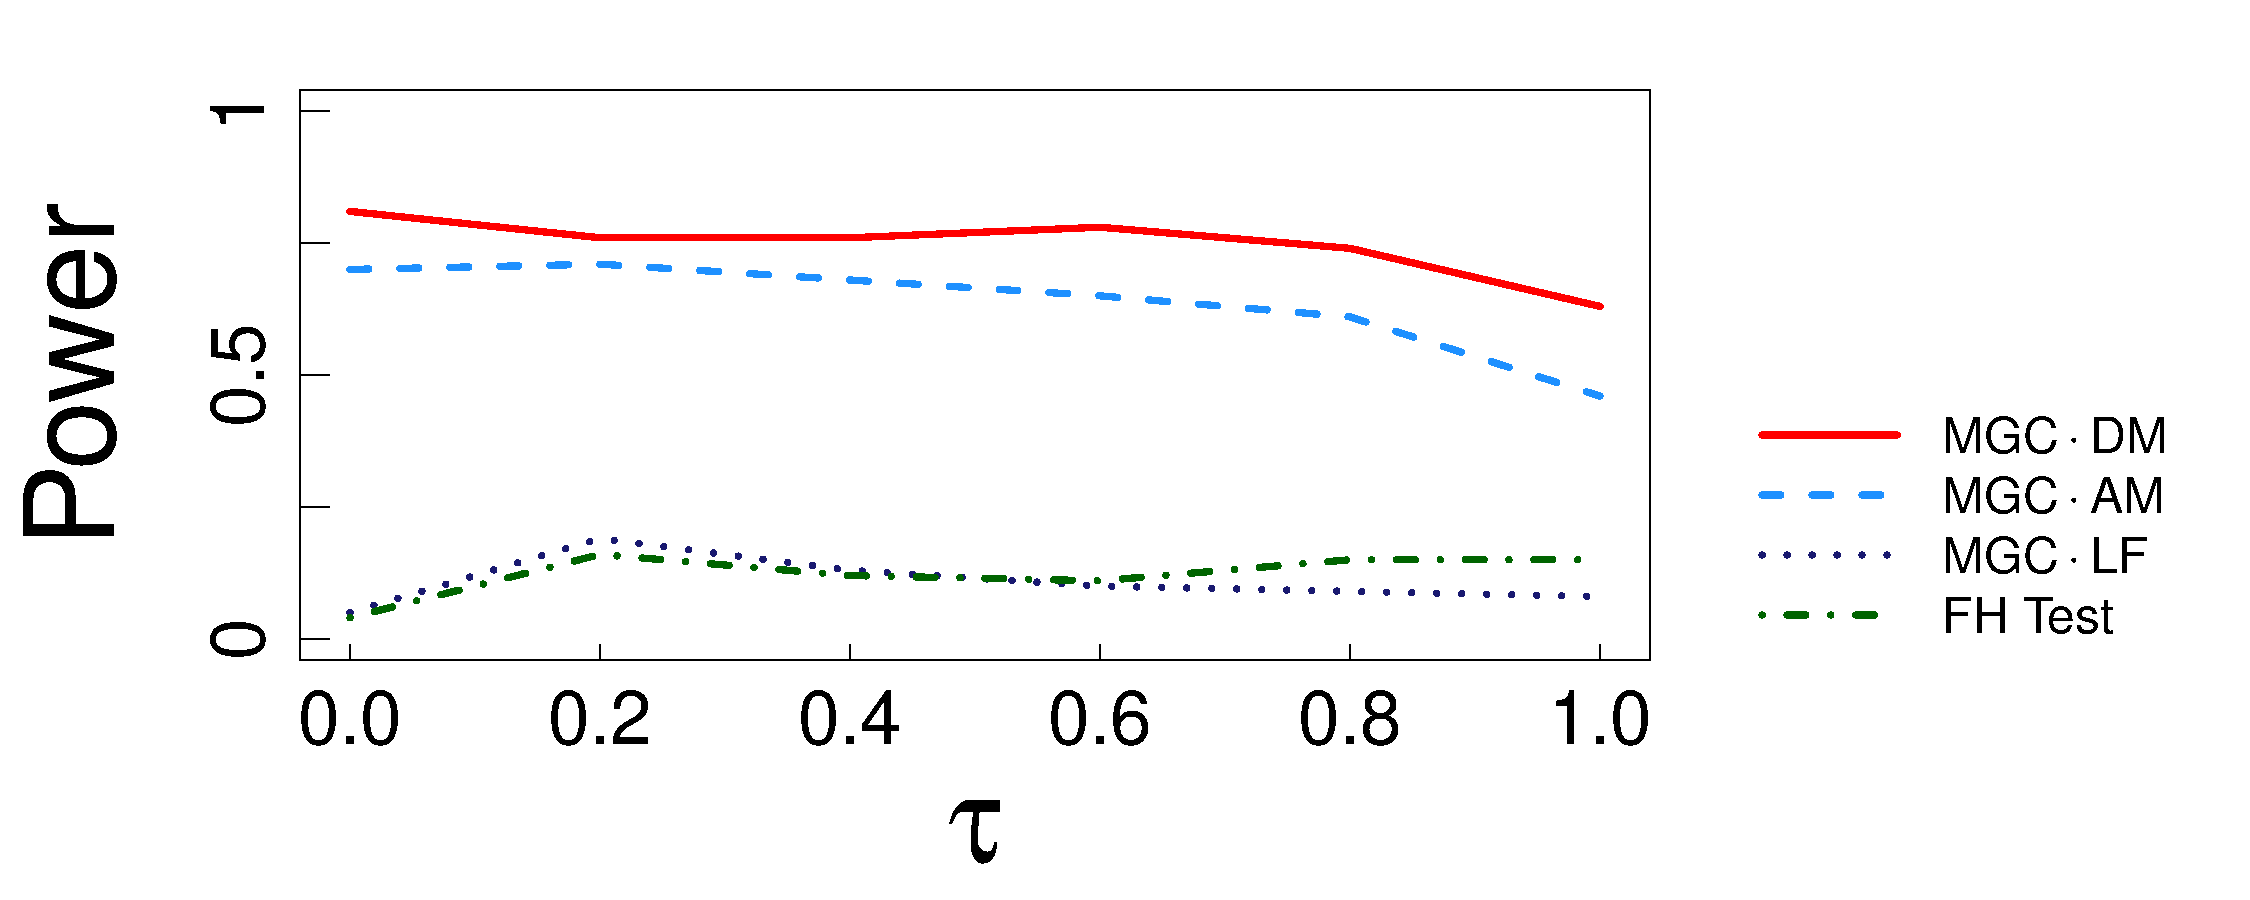
\includegraphics[width=\textwidth]{../Figure/elbow3_dcSBM.pdf}
		\caption{} 
		\label{fig:tau}
	\end{subfigure}
	\caption{ (Figure~\ref{fig:powerplot}) The power curve with respect to increasing $\theta$ under three-block SBM (Equation~\ref{eq:mono}) where $\{\theta : \theta \leq 0.2 \}$ represents a close to linear dependency between the adjacency matrix and the block structure; while $\{ \theta : \theta > 0.2 \}$ generates nonlinear dependency and it becomes strongly nonlinear as $\theta$ gets further away from $0.2$. Among other benchmarks utilizing diffusion maps, \texttt{MGC} is the best performing method throughout all possible $\theta$, implying that it is able to better capture nonlinear dependencies. (Figure~\ref{fig:tau}) The power curve with respect to increasing $\tau$ under DC-SBM (Equation~\ref{eq:tau}). As the edge variability increases as $\tau$ does, the testing power of diffusion maps are relatively stable against increasing variability compared to the adjacency matrix; while the latent positions fail to detect the dependency across all levels of $\tau$.} 
\end{figure}
\subsection{Degree-corrected Stochastic Block Model}
Next we investigate the degree-corrected stochastic block model (DC-SBM), which better reflects many sparse networks in reality. The DC-SBM is an extension of SBM by introducing an additional random variable $\mathbf{c}_{i}$ to control the degree of each node. 

We set $n=200$ and $K=2$, select the block membership $\mathbf{z}_i$ uniformly in $\Omega=\{0,1\}$, and generate the edge probability by  
\vspace*{-0.4cm}
\begin{equation}
E( \mathbf{A}_{ij} | \mathbf{z}_{i}, \mathbf{z}_{j},\mathbf{c}_{i},\mathbf{c}_{j} )  = 0.2 \mathbf{c}_{i} \mathbf{c}_{j} \cdot \mathbf{I}( |\mathbf{z}_{i} - \mathbf{z}_{j}| = 0 ) + 0.05 \mathbf{c}_{i} \mathbf{c}_{j} \cdot \mathbf{I}(|\mathbf{z}_{i} - \mathbf{z}_{j}| = 1),
\label{eq:tau}
\end{equation} 
where $\mathbf{c}_{i} \overset{i.i.d}{\sim} Uniform(1 - \tau, 1 + \tau)$ for $i = 1, \ldots, n$, and $\tau \in [0, 1]$ is a parameter to control the amount of variability in the edge degree, e.g., as $\tau$ increases, the model becomes more complex as the variability of the edge probability becomes larger; when $\tau=0$, the above model reduces to a two-block SBM without any variability induced by $\{ \mathbf{c}_{i} \}$. 

Similar as before, we generate the nodal attributes $\mathbf{X}$ as a noisy version of the true block memberships via Bernoulli distribution, i.e., for each $i$, $\mathbf{x}_{i}= \mathbf{z}_{i}$ with probability $0.6$, and equals the wrong label with probability $0.4$.

Under the DC-SBM model, the main approach also has the most superior power. In particular, Figure~\ref{fig:tau} compares different metrics using \texttt{MGC}, which illustrates that the diffusion map consistently reflect the network topology of DC-SBM better throughout different choices of $\tau$.

%\subsection{Random Dot Product Graph}
%\label{ssec:RDPG}

%Under the random dot product graph model (RDPG)~\cite{young2007random}, each node are assumed a latent position in Euclidean space, and the edge probability between node $i$ and $j$ is determined by the dot product of their latent positions. Denote $\{\mathbf{w}_{i} \in \mathbb{R}^{q_{x}} : i =1,2, \ldots, n \}$ as the latent position associated with each node, and assume that they are properly normalized with $\|\mathbf{w}_{i}\|_{2} \leq 1$ for all $i$ (such that the dot product $<\mathbf{w}_{i}, \mathbf{w}_{j} >$ never exceeds $1$). Then the edge $A_{ij}$ is determined by 
%\begin{equation}
%\begin{split}
%A_{ij} \big| \mathbf{w}_{i}, \mathbf{w}_{j}  \overset{i.i.d.}{\sim} Bernoulli \big( <\mathbf{w}_{i}, \mathbf{w}_{j} > \big), \quad \forall i < j.
%\end{split}
%\end{equation}

%In this experiment, we test dependency between a noisy version $\mathbf{X}$ of the latent positions and the graph adjacency $\mathbf{A}$ generated by the RDPG model, for which we set 
% and also additive multiplicative (AME) model of latent factors~\cite{fosdick2015testing}.
%$\mathbf{w}_{i} \overset{i.i.d.}{\sim} Uniform[0,1]$, $\mathbf{x}_{i} \sim Normal(\mathbf{w}_{i}, 0.5)$. %Note that this model is within the model assumption of the \texttt{FH} test~\cite{fosdick2015testing}.

%Figure~\ref{fig:RDPG} plots the testing power versus the sample size, where the \texttt{MGC} $\circ$

%actually illustrates that even in the case where the true data generating model obeys the additive and multiplicative model, when dimensional choice of latent factors depends on the result of elbow test, using \texttt{MGC} statistic combined with estimated latent factors (\texttt{LF}) performs better than the likelihood-based \texttt{FH} test; actually, this \texttt{FH} test even achieves less power than when the \texttt{MGC} is applied to diffusion maps which provide less accurate network metrics than the latent factors in this case.

%\begin{figure}[ht]
%	\centering
%	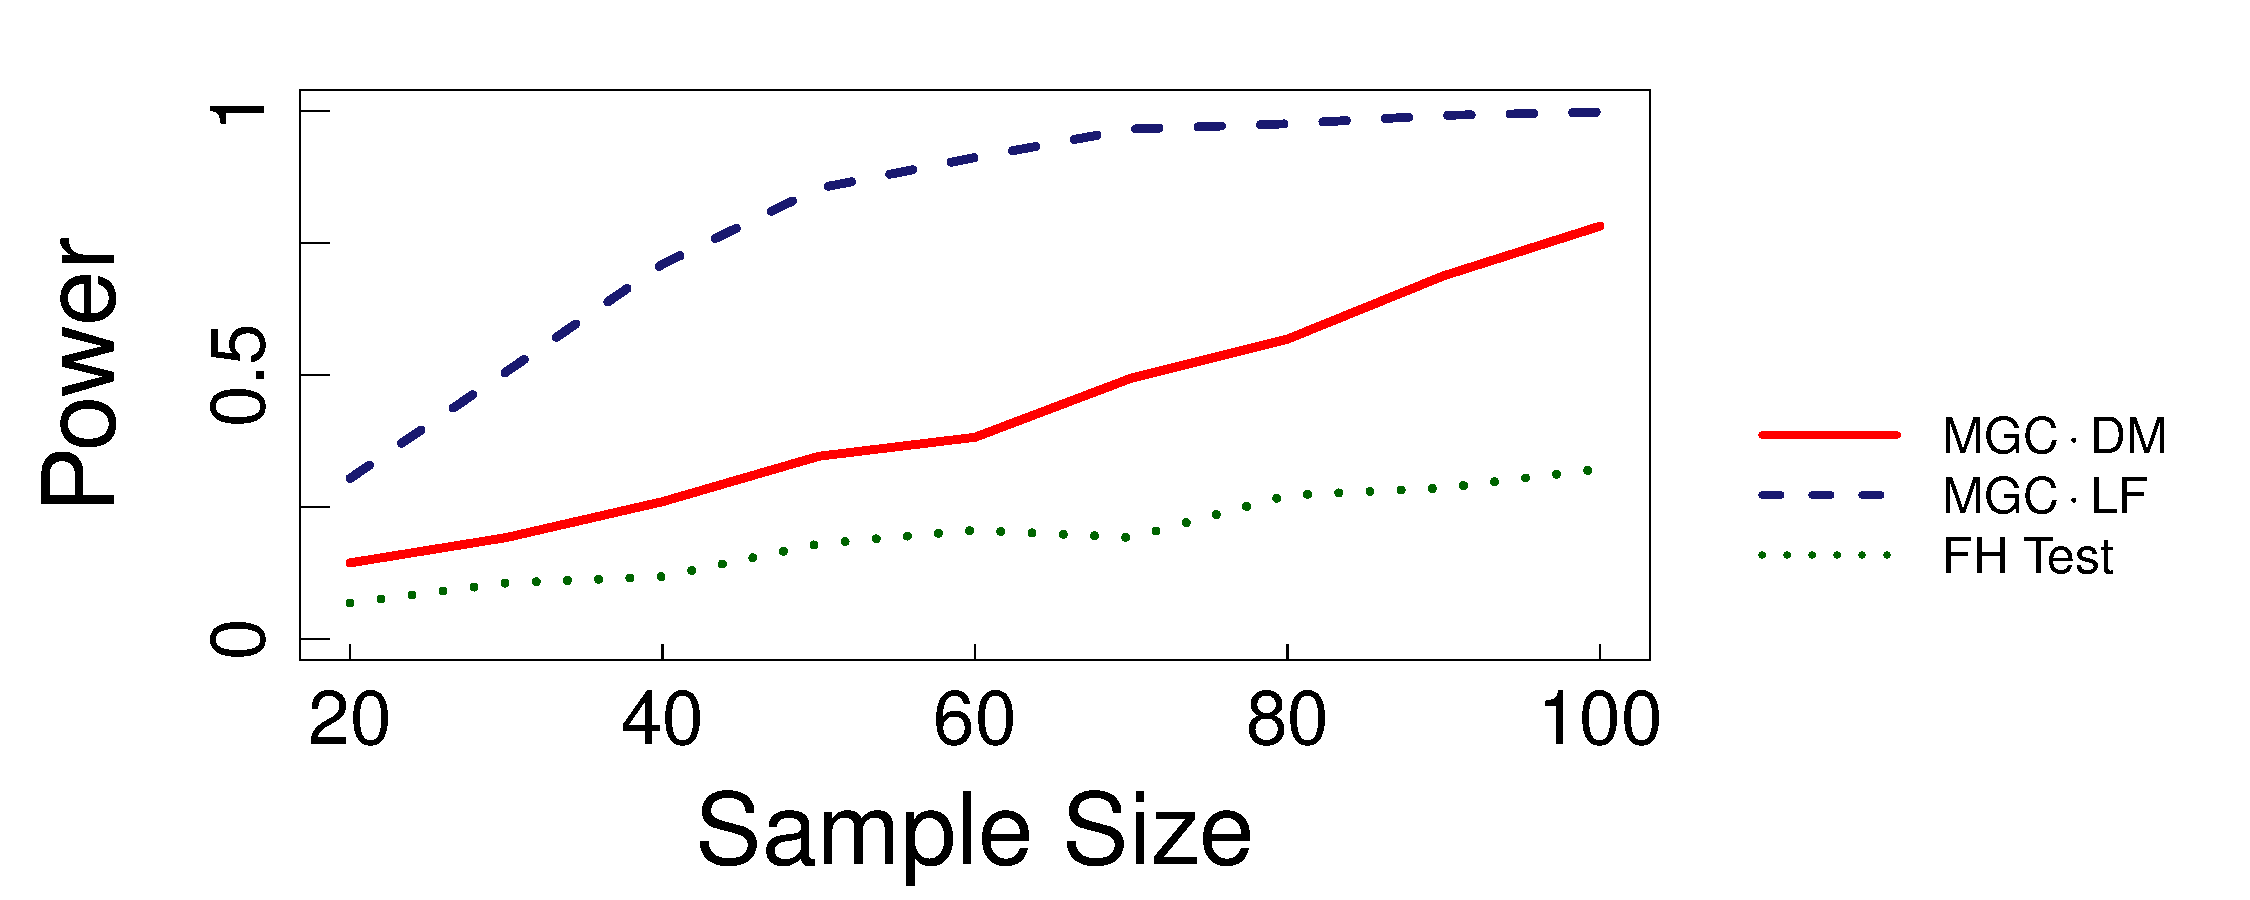
\includegraphics[width=0.7\linewidth]{elbow3_RDPG.pdf}
%	\caption{The third elbow has been applied in the choice of the dimension both for diffusion map (\texttt{DM}) and latent factor (\texttt{LF}) and the dimension of latent factors in \texttt{FH Test} and \texttt{MGC $\cdot$ LF} are identical. This figure shows that \texttt{MGC $\cdot$ LF} beats \texttt{FH Test} under the model~\ref{eq:RDPG}, where the additive and multiplicative model proposed by Fosdick and Hoff~\cite{fosdick2015testing} is close to the true data generating model.}
%	\label{fig:RDPG}
% \end{figure}

%%%%%%%%%%%%%%%%%%%%%%%%%%%%%%%%%%%%%%%%%
\subsection{Real Data Experiment}
\label{ssec:real}

To demonstrate the application of the proposed method in real data, we test independence on the brain network, where each node indicates voxel in the brain and edges represent brain fibers connecting each region~\cite{kiar2016ndmg}. Along with the information of the functional connectivity between the voxels, the data also provides the physical locations of each voxel in the brain represented by 3-dimensional voxel-wise coordinates. The brain network has been constructed by combining dMRI and sMRI data using the tool called \texttt{ndmg}~\cite{kiar2016science}, and the data is publicly available online \footnote{\url{http://openconnecto.me/data/public/MR/m2g_v1_1_1/KKI2009/derivatives/bg/}}.

The whole brain network data itself contains millions of nodes, so it is highly time-consuming to use all data for testing. As it is a common practice to sub-sample a small portion of big data for testing (under the assumption that significant relationship within the sub-sample is representative of the full data), we randomly selected one connected component having 95 nodes and 337 edges to test dependency between the functional connectivity versus each voxel's physical location. Moreover, we consider data contamination by edge flipping of the adjacency matrix: At contamination rate $c \%$, we randomly select $c \%$ of ones in the adjacency matrix and make them zeros, then randomly select $c \%$ of non-diagonal zeros and make them ones. Therefore, $c=0$ equals the original data, while $c=100$ flips all edges and is merely a transformation of the original graph.

Figure~\ref{fig:realexample} shows the p-value against the level of contamination $c \%$. The diffusion maps-based tests perform the best, with \texttt{MGC} and \texttt{mCorr} being slightly better than $\texttt{HHG}$. All other tests are less robust as the contamination level increases, e.g., \texttt{FH} test is able to yield a significant p-value at $c=0$, but fails at $c=100$ while the proposed approach is still able to test significant relationship. Note that there is only one p-value to report at $c=0$ and $c=100$, while at other choices of $c$ we randomly contaminate the data for $100$ replicates and report the mean p-value of them.

\begin{figure}[ht]
	\centering
	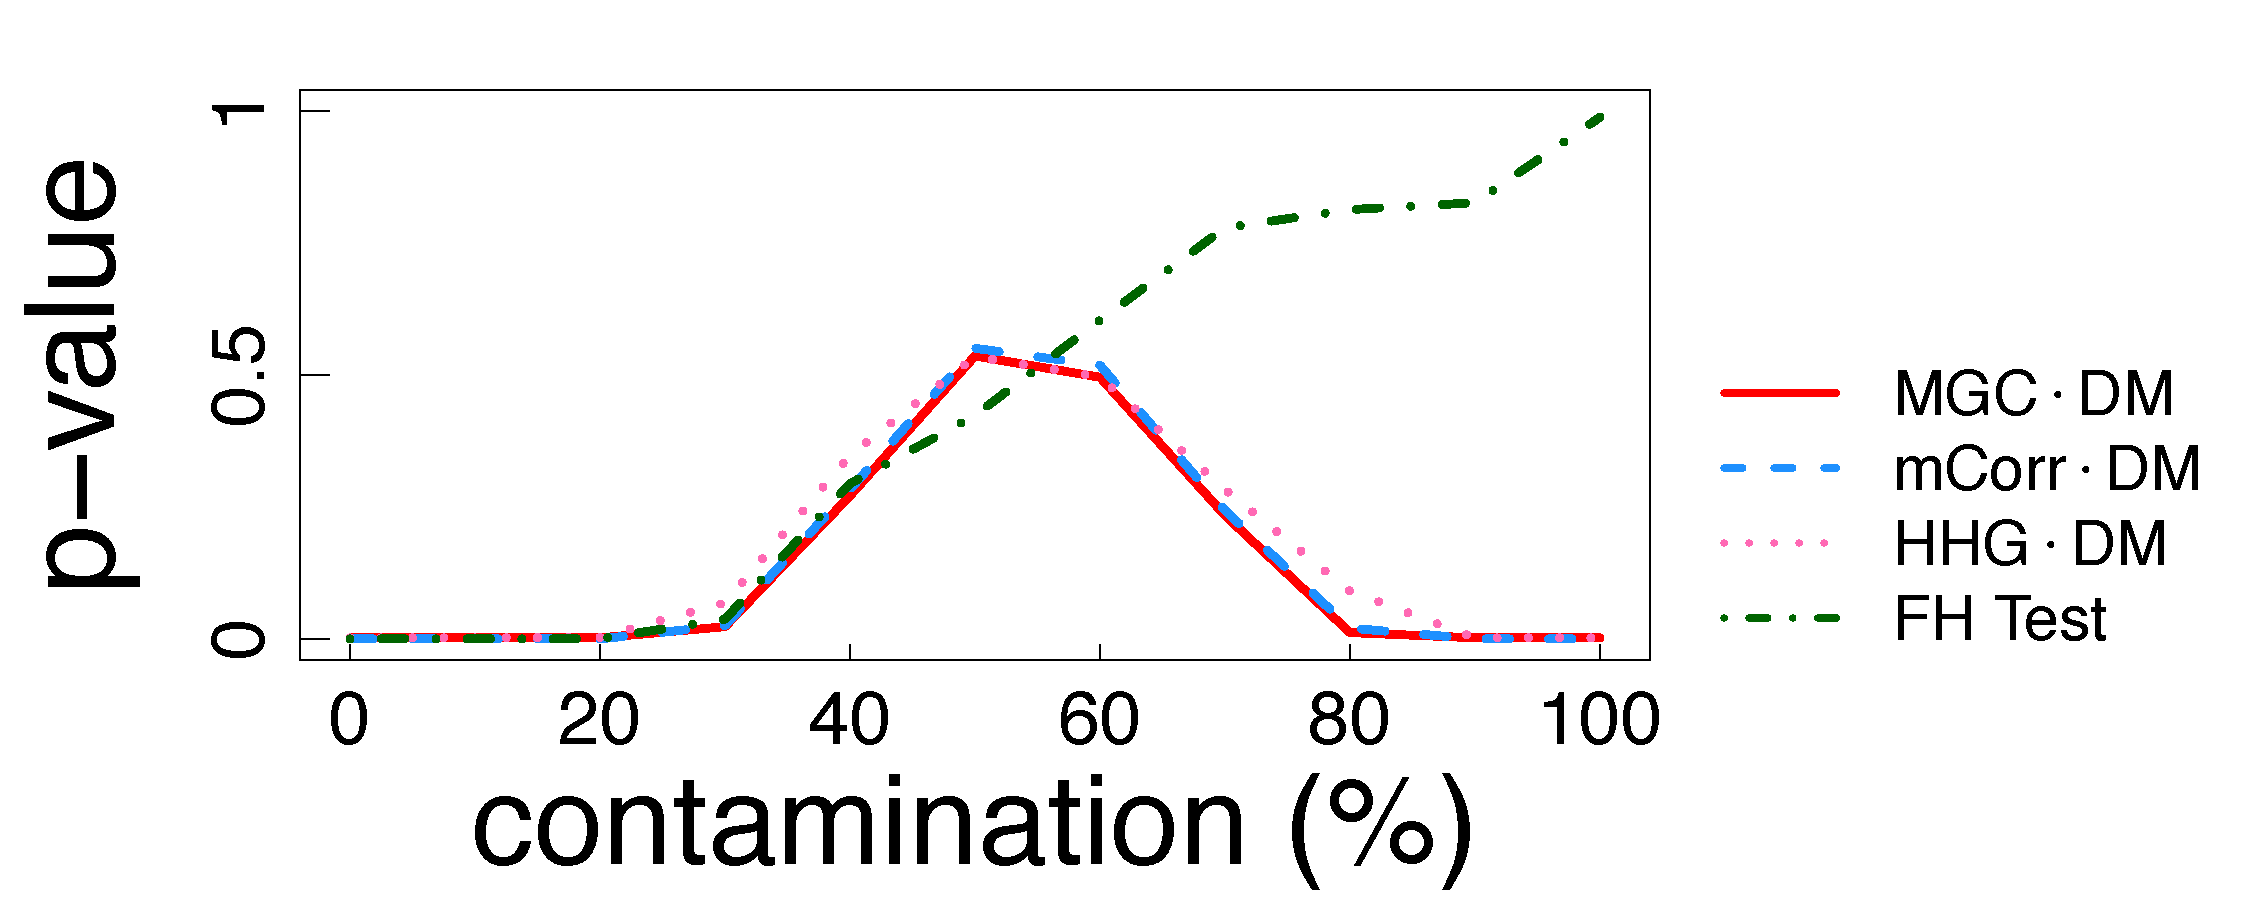
\includegraphics[width=0.7\textwidth]{../Figure/Elbow3_t3.pdf}
	\caption{P-values are obtained through 100 random contamination for each of $c\% \in \{ 10\%, 20\%, \ldots, 90\% \}$. As the level of contamination increases, it is less likely to reject the independence hypothesis with the \texttt{FH Test} than with our proposed approach.}
\label{fig:realexample}
\end{figure}

%%%%%%%%%%%%%%%%%%%%%%%%%%%%%%%%%%%%%%%%%
\section{Conclusion}
	\label{sec:conc}
	
In this study, we propose a new method for testing dependency on network data via diffusion maps and distance-based correlations. The utilization of the diffusion maps not only warrants the integration with various types of distance-based correlations, but also makes the testing method robust against parameter mis-specifications. Moreover, applying multiscale generalized correlation allows the test to detect a wide range of nonlinear, high-dimensional, and noisy dependencies. Therefore, the proposed approach is able to achieve significant power improvement over other alternatives in network dependency testing. 
    
There are several follow-ups that would further advance a number of frontiers in this area. First, it would be desirable to theoretically prove the robustness of the diffusion maps, and compare to other embedding methods under certain network models. Secondly, as network data in practice are often of huge size, the time and space requirement for dependence testing can be formidable without sub-sampling \cite{zhang2017large}, thus it would be necessary to further investigate the testing performance via sub-sampling. Third, it will be worthwhile to further investigate dependence testing or two-sample testing on two networks, in particular graphs with only partial correspondence. Last but not least, the framework proposed in this paper also defines a good correlation measure on networks, thereby enabling certain popular statistical techniques to be directly applied to network data such as feature screening via distance correlation \cite{LiZhongZhu2012}.

%%%%%%%%%%%%%%%%%%%%%%%%%%%%%%%%%%%%%%%%%%%%
\clearpage
\bibliographystyle{Chicago}
\bibliography{reference}

\section*{Acknowledgment}
% \addcontentsline{toc}{section}{Acknowledgment}
This work was partially supported by the
%
National Security Science and Engineering Faculty Fellowship (NSSEFF),
%
the Johns Hopkins University Human Language Technology Center of Excellence (JHU HLT COE),  the
%
Defense Advanced Research Projects Agency's (DARPA) SIMPLEX program through SPAWAR contract N66001-15-C-4041,
%
the XDATA program of DARPA administered through Air Force Research Laboratory contract FA8750-12-2-0303.
%
The authors thank Dr.~Daniel Sussman, Dr.~Minh Tang,  and Dr.~Carey Priebe for insightful suggestions.

%%%%%%%%%%%%%%%%%%%%%%%%%%%%%%%%%%%%%%%%%%%%%%
\clearpage
\appendix
\section{Proofs}
\label{ssec:proof}

%%%%%%%%%%%%%%%%%%%%%%%%%%%%%%%%%%%%%%%%	
\begin{proof}[\textbf{Proof of Theorem~\ref{main_lemma}}]
To prove conditional i.i.d. of the diffusion map $\mathbf{U} = \{\mathbf{u}_i : i=1,\ldots,n\}$ as $n \rightarrow \infty$, by the celebrated \textit{de Finetti's Theorem}~\cite{diaconis1980finite,orbanz2015bayesian} it is equivalent to prove that $\{ \mathbf{u}_i : i=1,\ldots,n \}$ are infinitely exchangeable, i.e., for any $n$ and all possible permutation $\sigma$, the permuted sequence $\{\mathbf{u}_{\sigma(1)}, \mathbf{u}_{\sigma(2)}, \ldots,\mathbf{u}_{\sigma(n)}\}$ always distributes the same as the original sequence $\{\mathbf{u}_{1}, \mathbf{u}_{2}, \ldots,\mathbf{u}_{n}\}$.

From now on, denote $\mathbf{U}$ as the $q \times n$ matrix having $\mathbf{u}_i$ as its $i^{th}$ column, and the permuted matrix as $\mathbf{U} \pi$ with $\pi$ being the permutation matrix. Transforming Equation~\ref{eq:U} into matrix notation yields
\begin{align*}
\mathbf{U}=\Lambda^{t}\Phi^{'},
\end{align*}
where $\Lambda=diag\{ \lambda_{1},\lambda_2,\ldots,\lambda_q \}$ is the diagonal matrix of selected eigenvalues of the transition matrix $\mathbf{\widetilde{K}}$; $\Phi =[ \mathbf{\phi}_1, \mathbf{\phi}_2,\cdots, \mathbf{\phi}_q ]$ consists of the corresponding eigenvectors; $\cdot^{t}$ denotes $t$th power; and $\cdot^{'}$ is the matrix transpose. Therefore, it suffices to show that $\mathbf{U}$ always distributes the same as $\mathbf{U} \pi$ for any $n$ and $\pi$.

Given that the graph $\mathbf{G}$ is infinitely exchangeable, i.e., $\mathbf{A}_{\sigma(i)\sigma(j)} \stackrel{d}{=} \mathbf{A}_{ij}$, we have
\begin{align*}
\mathbf{\widetilde{K}}_{\sigma(i) \sigma(j)} &= \max\{\mathbf{A}_{\sigma(i) \sigma(j)},\mathbf{A}_{\sigma(j) \sigma(i)}\} / \sum\limits_{j} \max\{\mathbf{A}_{\sigma(i) \sigma(j)},\mathbf{A}_{\sigma(j) \sigma(i)}\} \\
 &\stackrel{d}{=} \max\{\mathbf{A}_{ij},\mathbf{A}_{ji}\} / \sum\limits_{j} \max\{\mathbf{A}_{ij},\mathbf{A}_{ji}\} \\
&= \mathbf{\widetilde{K}}_{ij}.
\end{align*}
Thus the transition matrix $\mathbf{\widetilde{K}}$ is also infinitely exchangeable, i.e., $\pi^{'} \mathbf{\widetilde{K}} \pi \stackrel{d}{=} \mathbf{\widetilde{K}}$ for any permutation $\pi$ and any size $n$. 

By eigen-decomposition, the first $q$ eigenvectors and the corresponding eigenvalues of $\pi^{'} \mathbf{\widetilde{K}} \pi$ are $\Lambda$ and $\pi^{'} \Phi$, so it follows that
\begin{align*}
	& \Phi \stackrel{d}{=} \pi^{'} \Phi\\
        \Leftrightarrow \quad
        & \mathbf{U}=\Lambda^{t} \Phi^{'}  \stackrel{d}{=} \Lambda^{t} \Phi^{'} \pi = \mathbf{U} \pi 
\end{align*}	
Therefore, the diffusion maps are also infinitely exchangeable, and there exists a latent variable $u$ such that the diffusion map is conditional i.i.d. asymptotically. 
\end{proof}

%%%%%%%%%%%
\begin{proof}[\textbf{Proof of Lemma~\ref{main_lemma_1}}]
To prove that $u$ is of finite second moment, it suffices to show that $\|\mathbf{u}_{i}\|_{2}$ is always bounded for all $i \in [1,n]$.

By Equation~\ref{eq:U}, we have 
\begin{align*}
\| \mathbf{u}_i \|_{2}^{2}  &= \sum_{j=1}^{q} \lambda^{2t}_{j}\mathbf{\phi}_{j}^{2}(i) \\ 
& \leq \sum_{j=1}^{q} \lambda^{2t}_{j} \\
& \leq q,
\end{align*}
where the second line follows by noting $\mathbf{\phi}_{j}(i) \in [-1,1]$ (the eigenvector $\mathbf{\phi}_{j}$ is always of unit norm), and the third line follows by observing that $| \lambda_{j}| \leq \|\widetilde{\mathbf{K}}\|_{\infty}= 1$.

Therefore, all of $\mathbf{u}_{i}$ are bounded in $\ell_{2}$ norm as $n \rightarrow \infty$, so the latent variable $u$ must be of finite second moment.
\end{proof}

%%%%%%%%%%%%%%%%%%%%%%%
%%%%%%%%%%%%%%%%%%%%%%%%
\begin{proof}[\textbf{Proof of Theorem~\ref{theoremMain}}]

We first state two useful lemmas:
\begin{lemma}
	\label{lemma2}
	Let $\mathcal{V}^2_{n}(\mathbf{U}, \mathbf{X})$ be the distance covariance (\texttt{dCov}) of $(\mathbf{U}, \mathbf{X}) = \{  ( \mathbf{u}_{i}, \mathbf{x}_{i}  )  : i = 1, \ldots, n \}$ defined as Equation~\ref{eq:dCov}.
	It follows that
\begin{eqnarray}
		\mathcal{V}^{2}_{n}(\mathbf{U},\mathbf{X}) &=   \|g_{\mathbf{U},\mathbf{X}}^{n}(t,s)-g_{\mathbf{U}}^{n}(t)g_{\mathbf{X}}^{n}(s)\|^{2},
\end{eqnarray}
	where $g_{\cdot}^{n}$ is the empirical characteristic function of $\{(\mathbf{u}_{i},\mathbf{x}_{i}) : i=1,2,...,n\}$ or the marginals, e.g., $g_{\mathbf{U},\mathbf{X}}^{n}(t,s)=\frac{1}{n}\sum_{i=1}^{n}\exp\{i \left\langle t,\mathbf{u}_{i} \right\rangle+i \left\langle s,\mathbf{x}_{i} \right\rangle\}$, with the understanding that the $i$ before the inner product is the imaginary unit.
\end{lemma}

\begin{lemma}
	\label{lemma3}
	Assume $\{ \mathbf{u}_{i} : i = 1,2, \ldots, n \}$ are conditional i.i.d. based on $u$, and $\{\mathbf{x}_{i} \stackrel{i.i.d.}{\sim} x,~i = 1, 2, \ldots, n\}$, where $u$ and $x$ are both of finite second moment. It follows that
	\begin{eqnarray}
	\mathcal{V}_{n}^{2}(\mathbf{U},\mathbf{X}) &\longrightarrow \mathcal{V}^{2}(u,x) \quad \quad \mbox{ as } n \rightarrow \infty
	\label{eq:conv1}
	\end{eqnarray}
	where $\mathcal{V}^{2} (u,x) := \| g_{u,x}(t,s) - g_{u}(t) g_{x}(s) \|^2$, and $g_{\cdot}$ is the characteristic function, e.g., $g_{u,x}(t,s) = E(\exp\{i \left\langle t,u \right\rangle  +i \left\langle  s,x\right\rangle \})$.
\end{lemma}

By Theorem~\ref{main_lemma}, each observation in the diffusion map $\mathbf{U}$ is asymptotic i.i.d. conditioned on $u$ under an infinitely exchangeable graph, while the nodal attributes $\mathbf{X}$ are assumed i.i.d. as $x$. The finite moment of $u$ is guaranteed by Lemma~\ref{main_lemma_1}, and the finite moment of $x$ is assumed in (C2).

Therefore a direct application of Lemma~\ref{lemma2} and Lemma~\ref{lemma3} yields that
\begin{eqnarray}
\mbox{\texttt{dCov}}(\mathbf{U},\mathbf{X}) &\longrightarrow \| g_{u,x}(t,s) - g_{u}(t) g_{x}(s) \|^2,
\end{eqnarray}
which equals $0$ if and only if $u$ is independent of $x$.

As distance correlation is just a normalized version of distance covariance, it further leads to
\begin{eqnarray}
\mbox{\texttt{dCorr}}(\mathbf{U},\mathbf{X}) &\longrightarrow 0,
\label{eq:main1}
\end{eqnarray}
if and only if independence.

By \cite{shen2016discovering}, whenever Equation~\ref{eq:main1} holds for \texttt{dCorr}, it automatically holds for \texttt{MGC}. Therefore, \texttt{MGC} is consistent for testing dependence between the diffusion maps $\mathbf{U}$ and the nodal attributes $\mathbf{X}$.
\end{proof}

\begin{proof}[\textbf{Proof of Lemma~\ref{lemma2}}] 
This lemma follows exactly from Theorem 1 in \cite{szekely2007measuring}, which holds without any assumption on $(\mathbf{U}, \mathbf{X} ) =  \{(\mathbf{u}_{i},\mathbf{x}_{i}) :  i=1,2,...,n\}$, e.g., it holds without assuming exchangeability, nor identically distributed, nor finite second moment.
\end{proof}

\begin{proof}[\textbf{Proof of Lemma~\ref{lemma3}}] 
The conclusion of this lemma is equivalent to Theorem 2 in \cite{szekely2007measuring}. The only difference is that the original set-up assumes $\{(\mathbf{u}_{i},\mathbf{x}_{i}) : i = 1, \ldots , n \}$ is independently identically distributed as $(u,x)$ with finite second moment; while here $\{  \mathbf{u}_{i} : i = 1, \ldots, n  \}$ is asymptotic conditionally i.i.d. and of finite second moment.

All major steps in proving Theorem 2 of \cite{szekely2007measuring} are essentially the same for either i.i.d. random variables or infinitely exchangeable random variables. In particular, under the finite second moment assumption, we still have the strong large number for V-statistics \cite{KoroljukBook}, i.e., 
	\begin{eqnarray}
	\displaystyle\int_{D(\delta)}{\|g_{u,x}^{n}(t,s)-g_{u}^{n}(t)g_{x}^{n}(s)\|^{2}}dh &\stackrel{n \rightarrow \infty}{\longrightarrow} 
	\displaystyle\int_{D(\delta)}{\|g_{u,x}(t,s)-g_{u}(t)g_{x}(s)\|^{2}}dh,
	\label{eq:SLLN}
	\end{eqnarray}
	where $D(\delta)=\{(t,s):\delta \leq |t|_{p} \leq 1/\delta,\delta \leq |s|_{q} \leq 1/\delta\}$, and $h(t,s)$ is a weight function chosen in \cite{szekely2007measuring}. 
\end{proof}

\begin{proof}[\textbf{Proof of Corollary~\ref{main_corollary}}] 
(1) All the proofs remain the same regardless of the choice of $t$ and $q$, as long as they are finite positive integers.

(2) When the nodal attribute is replaced by a second graph with the same node set as the first graph, we simply compute the diffusion map of the second graph by the same procedure as for the first graph. The resulting diffusion map of the second graph clearly satisfies both Theorem~\ref{main_lemma} and Lemma~\ref{main_lemma_1}, and the proof of Theorem~\ref{theoremMain} works for two asymptotic conditional i.i.d. latent variables without any change.

(3) Changing the test statistic only affects Theorem~\ref{theoremMain}, for which Equation~\ref{eq:main1} is the key step. As \texttt{mCorr} converges to \texttt{dCorr} by \cite{szekely2013distance}, Equation~\ref{eq:main1} also holds for \texttt{mCorr}. It has been further shown in \cite{shen2016discovering} that \texttt{MGC} satisfies the same equation whenever it holds for the respective global correlation. 
\end{proof}

\end{document}